\documentclass[a5paper, 10pt, twoside, bahasa]{report}
\title{Tugas Akhir - Deteksi Jatuh}
\usepackage{graphicx}
\usepackage{hyphenat}
\usepackage{comment}
\usepackage{array}
\usepackage{multirow}
\usepackage{rotating}
\usepackage{booktabs}
\usepackage[ruled,lined,commentsnumbered,linesnumbered]{algorithm2e}
\usepackage{algpseudocode}
\usepackage{makeidx}
\makeindex
\usepackage[pdfauthor={Rohman Widiyanto},bookmarksnumbered,pdfborder={0 0 0}]{hyperref}  
\usepackage[indonesian]{babel}
\usepackage{epsfig}
\usepackage{subfig}
\usepackage[top=25mm,left=25mm,right=20mm,bottom=25mm]{geometry}
\usepackage{pdflscape}
\usepackage{setspace}  
\usepackage{type1cm}
\usepackage{lettrine}
\usepackage{hyperref}
\usepackage[pageref]{backref}
\usepackage{multirow}
\usepackage{fancyhdr} 		% Untuk pengaturan header dan footer yang lebih kompleks
\usepackage{etoolbox} 		% Untuk melakukan perubahan (patch) command internal LaTeX
\usepackage{url}
\usepackage{longtable}
\usepackage{float}
\floatstyle{boxed}
\newfloat{program}{thp}{lop}
\floatname{program}{Program}
\usepackage[fleqn]{amsmath}
\usepackage{enumitem}
\usepackage{nonfloat}
\usepackage{ulem}
\usepackage[final]{pdfpages}
\usepackage [raggedright]{titlesec}

\usepackage{array}
\usepackage{multicol}
\usepackage{listings}
\usepackage{wrapfig}

% Caption label bold
\usepackage[labelfont=bf]{caption}
\captionsetup{labelfont=bf}

% Jarak caption dengan obyek
\captionsetup[figure]{font=small,skip=5pt}
\captionsetup[table]{font=small,skip=5pt}
\captionsetup[lstlisting]{font=small,skip=5pt}

% Caption nama
\renewcommand{\figurename}{Gambar}
\renewcommand{\tablename}{Tabel}
\renewcommand{\lstlistingname}{Kode}

% Buat source code
\usepackage{courier}
\lstset{
	% language=C++, 						% Bahasa pengrograman yang digunakan
	basicstyle=\ttfamily \footnotesize,	% Jenis font dalam listing & Ukuran font
	% numbers=left, 						% Posisi angka untuk line-number
	% numberstyle=\footnotesize, 		% Ukuran angka untuk line-numbers
	% stepnumber=1, 						% Jarak setiap line-numbers
	% numbersep=5pt, 					% Ukuran line-numbers
	backgroundcolor=\color{white}, 		% Warna background. Gunakan \usepackage{color} dulu
	showspaces=false, 					% Show spaces adding particular underscores
	showstringspaces=false, 				% Underline spaces within strings
	showtabs=false, 						% Show tabs within strings adding particular underscores
	frame=single, 						% Tambahkan Frame
	framesep=0.1pt,						% Jarak frame dengan list content keseluruhan
	framexbottommargin=4pt,				% Jarak frame dengan list content bawah
  	framextopmargin=4pt,					% Jarak frame dengan list content atas
  	framexleftmargin=0pt,				% Jarak frame dengan list content kiri
  	framexrightmargin=0pt,				% Jarak frame dengan list content kanan
	tabsize=2, 							% Sets default tabsize to 2 spaces
	captionpos=b,						% Posisi caption
	breaklines=true, 					% Line breaking
	breakatwhitespace=false, 			% Sets if automatic breaks should only happen at whitespace
	escapeinside={\%*}{*)}				% if you want to add a comment within your code
}

% Untuk cek nomor halaman
\usepackage{changepage}
\usepackage{graphicx}

%Untuk check mark dan x-mark
\usepackage{amssymb}% http://ctan.org/pkg/amssymb
\usepackage{pifont}% http://ctan.org/pkg/pifont
\newcommand{\cmark}{\ding{51}}%
\newcommand{\xmark}{\ding{55}}%

\usepackage{lipsum}
\hyphenation{meng-gerak-kan mem-per-kenal-kan me-nger-ja-kan sa-ran seg-men be-ru-pa rasp-ber-ry meng-hu-bun-kan ter-sim-pan smart-phone me-nya-ma-kan sin-kro-ni-sa-si ke-ce-pa-tan di-hu-bung-kan sam-bu-ngan me-ru-pa-kan meng-gu-na-kan ber-da-sar-kan di-la-ku-kan di-gu-na-kan di-ban-ding-kan}

% Definisi untuk "halaman sengaja dikosongkan"
\def\kosong{
  \vspace*{\fill}
  \begin{center}\textit{Halaman ini sengaja dikosongkan}\end{center}
  \vfill
}
\patchcmd{\cleardoublepage}{\hbox{}}{\kosong}{}{}

% Tambahkan PDF atau Gambar
\newif\ifpdf
\ifx\pdfoutput\undefined
   \pdffalse
\else
   \pdfoutput=1
   \pdftrue
\fi
\ifpdf
   \usepackage{graphicx}
   \usepackage{epstopdf}
   \DeclareGraphicsRule{.eps}{pdf}{.pdf}{`epstopdf #1}
   \pdfcompresslevel=9
\else
   \usepackage{graphicx}
\fi

% utk itemize yg lebih rapat
\newenvironment{packed_enum}{
\begin{enumerate}[nolistsep]
  \setlength{\itemsep}{0pt}
  \setlength{\parskip}{0pt}
  \setlength{\parsep}{0pt}
}{\end{enumerate}}

% Untuk citation
\newcommand{\tab}[1]{\hspace{.2\textwidth}\rlap{#1}}
\renewcommand*{\backreflastsep}{, }
\renewcommand*{\backreftwosep}{, }
\renewcommand*{\backref}[1]{}
\renewcommand*{\backrefalt}[4]{
  \ifcase #1
    No citations.
  \or
    (Dikutip pada halaman #2).
  \else
    (Dikutip pada halaman #2).
  \fi
}

% Pengaturan penomoran halaman menggunakan package fancyhdr
\fancyhf{} 								% Mengosongkan header dan footer
\renewcommand{\headrulewidth}{0pt} 		% Menghapus garis horizontal pada header
\pagestyle{fancy} 						% Mengubah pagestyle dokumen menjadi fancy
\fancyfoot[CE,CO]{\thepage}				% Footer kanan pada hal. ganjil dan sebaliknya
\patchcmd{\chapter}{plain}{fancy}{}{} 	% Mengubah pagestyle pada chapter menjadi fancy
\patchcmd{\chapter}{empty}{plain}{}{}

% Pengaturan format Chapter dan Section
\titleformat{\chapter}[display]{\bfseries\Large}{BAB \centering\thechapter}{0ex}{\vspace{0ex}\centering}[\vspace{0ex}]
\titleformat{\section}{\bfseries\large}{\MakeUppercase{\thesection}}{1ex}{}
\titlespacing*{\chapter}{0pt}{-4ex}{0pt}
\titlespacing{\section}{0pt}{0pt}{0pt}

\begin{document}
\singlespacing

% Sampul luar
\AddToShipoutPictureBG*{
  \AtPageLowerLeft{
    % Ubah nilai berikut jika posisi horizontal background tidak sesuai
    \hspace{-3.5mm}

    % Ubah nilai berikut jika posisi vertikal background tidak sesuai
    \raisebox{0mm}{
      
\includegraphics[width=\paperwidth,height=\paperheight]{sampul/sampul-luar.png}
    }
  }
}

% Menyembunyikan nomor halaman
\thispagestyle{empty}

% Pengaturan margin untuk menyesuaikan konten sampul
\newgeometry{top=95mm,left=25mm,right=20mm,bottom=25mm}

\begin{flushleft}

  % Pengaturan jenis dan warna teks yang digunakan
  \sffamily\color{white}

  % Ubah penomoran buku berikut sesuai dengan yang ditentukan oleh departemen
  \noindent\textbf{TUGAS AKHIR - EC184801}
  \vspace{6ex}

  % Ubah kalimat berikut sesuai dengan judul tugas akhir
  \noindent{\large \textbf{DETEKSI JATUH PADA MANUSIA LANJUT USIA BERBASIS 3D - CNN PADA SISTEM TERTANAM}}
  \vspace{4ex}

  % Ubah kalimat berikut sesuai dengan nama mahasiswa
  \noindent\textbf{Hafizh Fauzan} \\
  % Ubah kalimat berikut sesuai dengan NRP mahasiswa
  \textbf{NRP 0721 17 4000 0019}
  \vspace{2ex}

  \noindent\textbf{Dosen Pembimbing} \\
  % Ubah kalimat berikut sesuai dengan nama-nama dosen pembimbing
  \textbf{Dr. Reza Fuad Rachmadi, S.T., M.T.} \\
  \textbf{Arief Kurniawan, ST., MT.}
  \vspace{6ex}

  % Ubah kalimat berikut sesuai dengan nama departemen
  \noindent\textbf{DEPARTEMEN TEKNIK KOMPUTER} \\
  % Ubah kalimat berikut sesuai dengan nama fakultas
  \textbf{Fakultas Teknologi Elektro dan Informatika Cerdas} \\
  \textbf{Institut Teknologi Sepuluh Nopember} \\
  % Ubah kalimat berikut sesuai dengan tempat dan tahun pembuatan buku
  \textbf{Surabaya 2021}

\end{flushleft}

\restoregeometry
\cleardoublepage

% Nomor halaman pembuka dimulai dari sini
\pagenumbering{roman}

% Sampul dalam
\AddToShipoutPictureBG*{
  \AtPageLowerLeft{
    % Ubah nilai berikut jika posisi horizontal background tidak sesuai
    \hspace{-3.5mm}

    % Ubah nilai berikut jika posisi vertikal background tidak sesuai
    \raisebox{0mm}{
      
\includegraphics[width=\paperwidth,height=\paperheight]{sampul/sampul-dalam.png}
    }
  }
}

% Menyembunyikan nomor halaman
\thispagestyle{empty}

% Pengaturan margin untuk menyesuaikan konten sampul
\newgeometry{top=95mm,left=25mm,right=20mm,bottom=25mm}

\begin{flushleft}

  % Pengaturan jenis teks yang digunakan
  \sffamily

  % Ubah penomoran buku berikut sesuai dengan yang ditentukan oleh departemen
  \noindent\textbf{TUGAS AKHIR - EC184801}
  \vspace{6ex}

  % Ubah kalimat berikut sesuai dengan judul tugas akhir
  \noindent{\large \textbf{DETEKSI JATUH PADA MANUSIA LANJUT USIA BERBASIS 3D - CNN PADA SISTEM TERTANAM}}
  \vspace{4ex}

  % Ubah kalimat berikut sesuai dengan nama mahasiswa
  \noindent\textbf{Hafizh Fauzan} \\
  % Ubah kalimat berikut sesuai dengan NRP mahasiswa
  \textbf{NRP 0721 17 4000 0019}
  \vspace{2ex}

  \noindent\textbf{Dosen Pembimbing} \\
  % Ubah kalimat berikut sesuai dengan nama-nama dosen pembimbing
  \textbf{Dr. Reza Fuad Rachmadi, S.T., M.T.} \\
  \textbf{Arief Kurniawan, ST., MT.}
  \vspace{6ex}

  % Ubah kalimat berikut sesuai dengan nama departemen
  \noindent\textbf{DEPARTEMEN TEKNIK KOMPUTER} \\
  % Ubah kalimat berikut sesuai dengan nama fakultas
  \textbf{Fakultas Teknologi Elektro dan Informatika Cerdas} \\
  \textbf{Institut Teknologi Sepuluh Nopember} \\
  % Ubah kalimat berikut sesuai dengan tempat dan tahun pembuatan buku
  \textbf{Surabaya 2021}

\end{flushleft}

\restoregeometry
\cleardoublepage

% Sampul inggris
% \input{sampul/sampul-inggris.tex}
% \cleardoublepage

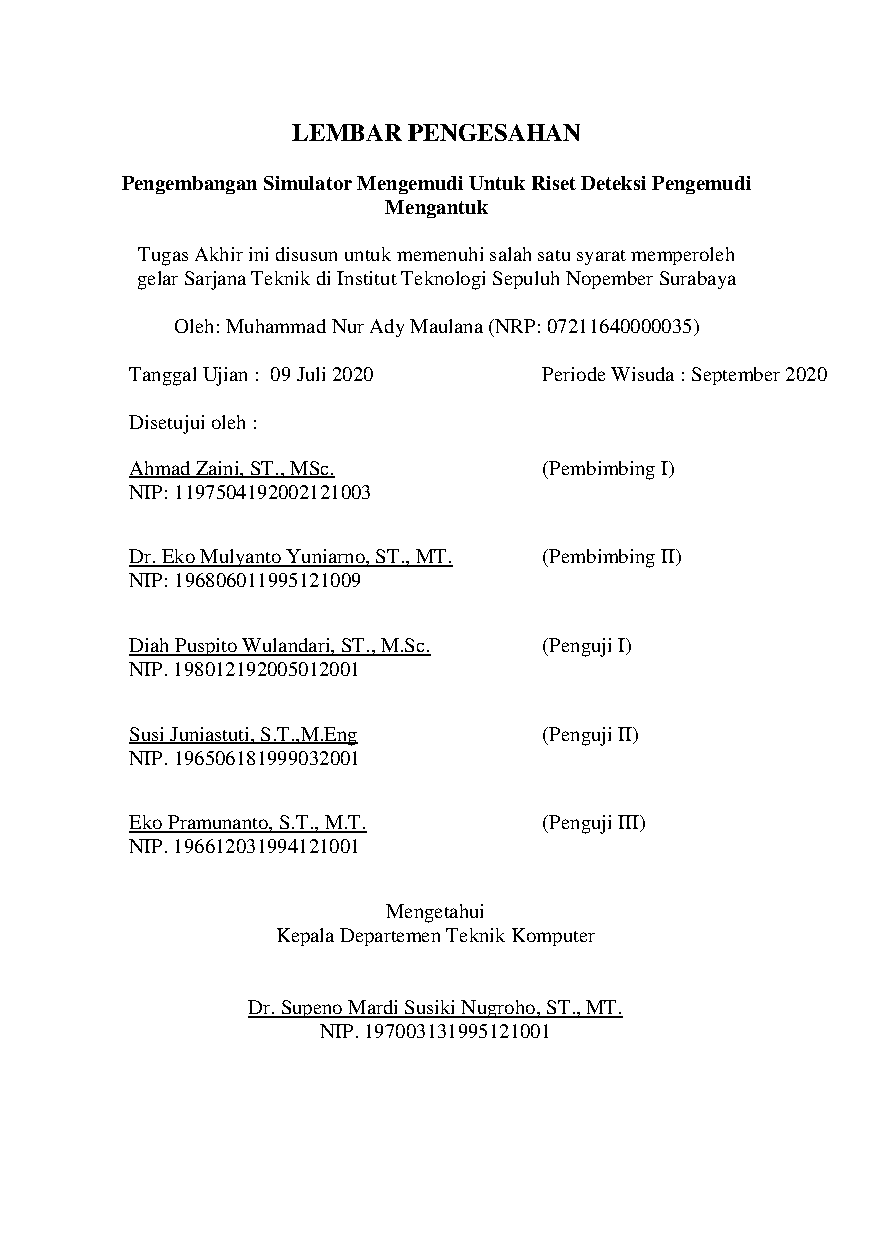
\includepdf[pages=-, offset=0 0]{file/Pengesahan.pdf}


% Abstrak bahasa indonesia
\addcontentsline{toc}{chapter}{Abstrak}
\begin{center}
\Large\textbf{ABSTRAK}
\end{center}
\vspace{1ex}

\begin{adjustwidth}{-0.2cm}{}
\begin{tabular}{lcp{0.6\linewidth}}
Nama Mahasiswa &:& Hafizh Fauzan \\
Judul Tugas Akhir &:& Deteksi Jatuh pada Manusia Lanjut Usia Berbasis 3D - CNN pada Sistem Tertanam\\
Pembimbing &:& 1. Dr. Reza Fuad Rachmadi, S.T., M.T. \\
& & 2. Arief Kurniawan, ST., MT.\\
\end{tabular}
\end{adjustwidth}
\vspace{1ex}

\setlength{\parindent}{0cm} Jatuh adalah penanda kelemahan, imobilitas, dan gangguan kesehatan akut dan kronis pada orang tua. Bahkan ketika cederanya tidak begitu serius, lansia seringkali kesulitan untuk bangkit tanpa bantuan ,terkadang mengarah ke 'long-lie' di mana lansia tetap terjebak di lantai untuk periode waktu yang lama. 'Long-lie' dapat menyebabkan dehidrasi, \textit{Ulkus dekubitus}, pneumonia, hipotermia dan kematian. Pada Tugas Akhir ini akan dikembangkan sebuah sistem yang dapat mendeteksi jatuh pada manusia lanjut usia menggunakan algoritma \textit{3D Convolutional Neural Network} berbasis sistem tertanam. Adapun training data yang digunakan berasal dari beberapa dataset publik dan akan dibuat dataset pribadi untuk testing dan revisi sistem. Hasil yang diharapkan melalui Tugas Akhir ini adalah terciptanya sebuah sistem pendeteksi jatuh yang dapat melakukan kontak dengan keluarga dan rumah sakit jika diperlukan apabila terdeteksi jatuh sehingga penderita dapat mengalami penanganan medis dengan cepat.


\vspace{2ex}

Kata Kunci : Jatuh, Deteksi, Sistem
\newpage
\cleardoublepage

% Abstrak bahasa ingris
%\addcontentsline{toc}{chapter}{Abstract}
%\begin{center}
\Large\textbf{ABSTRACT}
\end{center}
\vspace{1ex}

\begin{adjustwidth}{-0.2cm}{}
\begin{tabular}{lcp{0.6\linewidth}}
\textit{Name} &:& Nama\\
\textit{Title} &:& \textit{Title} \\
\textit{Advisors} &:& 1. Pembimbing1 \\
& & 2. Pembimbing2 \\
\end{tabular}
\end{adjustwidth}
\vspace{1ex}

	\setlength{\parindent}{0cm} Explain
	\vspace{2ex}
	
	\textit{Keywords : Train, Digital Map, Path Index, Speed Limit, Early Warning}
	\newpage

%\cleardoublepage

% Kata pengantar
\addcontentsline{toc}{chapter}{KATA PENGANTAR} % kata pengantar
\begin{center}
\Large\textbf{KATA PENGANTAR}
\end{center}
\vspace{1ex}

\setlength{\parindent}{0.9cm} Puji dan syukur kehadirat Tuhan Yang Maha Esa atas segala karunia-Nya, penulis  dapat menyelesaikan penelitian ini dengan judul \textbf{Pengembangan Simulator Mengemudi Untuk Riset Deteksi Pengemudi Mengantuk \textit{(Driving Simulator Development for Drowsy Driver Detection Research)}
}.
\vspace{1ex}

Penelitian ini disusun dalam rangka pemenuhan bidang riset di Departemen Teknik Komputer ITS, Bidang  Studi \textit{Game Technology}, serta digunakan sebagai persyaratan menyelesaikan pendidikan  S1. Oleh karena itu, penulis mengucapkan terima kasih kepada:
\vspace{1ex}

\begin{enumerate}[nolistsep]
  \item Bapak, ibu, adik, dan keluarga saya, atas semangat dan dukungan untuk tetap berkuliah
  \item Bapak Dr. Reza Fuad Rachmadi, S.T., M.T.
  \item Bapak Arief Kurniawan, ST., MT.
  \item Bapak - Ibu dosen pengajar Departemen Teknik Komputer, atas pengajaran, bimbingan, serta perhatian yang diberikan kepada penulis selama ini.
  \item Teman - teman Asisten Lab B201 Telematika yang selalu membantu dan menemani
  \item Teman - teman UKM Kendo ITS yang selalu memberi semangat
  \item Serta teman - teman angkatan 2017 yang telah bersama - sama melalui kehidupan perkuliahan bersama penulis
\end{enumerate}
\vspace{1ex}

Kesempurnaan hanya milik Allah SWT, untuk itu penulis memohon segenap kritik dan saran yang  membangun. Semoga penelitian ini dapat memberikan manfaat bagi kita semua. Amin.
\begin{flushright}
\begin{tabular}[b]{c}
  Surabaya, Juni 2021
  \\
  \\
  Penulis
\end{tabular}
\end{flushright}
\cleardoublepage

% Daftar isi
\renewcommand*\contentsname{DAFTAR ISI}
\addcontentsline{toc}{chapter}{\contentsname}
\titlespacing*{\chapter}{0pt}{-4ex}{2ex}
\tableofcontents	
\cleardoublepage

% Daftar gambar
\renewcommand*\listfigurename{DAFTAR GAMBAR}
\addcontentsline{toc}{chapter}{\listfigurename}
\titlespacing*{\chapter}{0pt}{-4ex}{2ex}
\listoffigures
\cleardoublepage

% Daftar tabel
\renewcommand*\listtablename{DAFTAR TABEL}
\addcontentsline{toc}{chapter}{\listtablename}
\titlespacing*{\chapter}{0pt}{-4ex}{2ex}
\listoftables
\cleardoublepage

% Nomenklatur
\addcontentsline{toc}{chapter}{NOMENKLATUR}
\begin{center}
	\Large\textbf{NOMENKLATUR}
\end{center}
\vspace{1ex}

\begin{tabular}{c m{30em}}
	$fps$	& : \textit{Frame Per Second} / Jumlah Citra Perdetik\\
	$unit$	& : unit pengukuran \textit{Unity Game Engine} \\
	
	
\end{tabular}
\vspace{1ex}
\cleardoublepage

% BAB isi buku
\titleformat{\chapter}[display]{\bfseries\Large}{BAB \centering\thechapter}{0ex}{\vspace{0ex}\centering}[\vspace{0ex}]
\titleformat{\section}{\bfseries\large}{\MakeUppercase{\thesection}}{1ex}{}
\titleformat{\subsection}{\bfseries\large}{\MakeUppercase{\thesubsection}}{1ex}{}
\titleformat{\subsubsection}{\bfseries\large}{\MakeUppercase{\thesubsubsection}}{1ex}{}
\titlespacing*{\chapter}{0pt}{-4ex}{0pt}
\titlespacing{\section}{0pt}{0pt}{0pt}
\titlespacing{\subsection}{0pt}{0pt}{0pt}
\titlespacing{\subsubsection}{0pt}{0pt}{0pt}

% Indent paragraph
\setlength{\parindent}{0.8cm}

% Penambahan halaman kosong otomatis
\chapter{PENDAHULUAN}
\pagenumbering{arabic}
\vspace{1ex}

\section*{}
Penelitian ini di latar belakangi oleh berbagai kondisi yang menjadi acuan. Selain itu juga terdapat beberapa permasalahan yang akan dijawab sebagai luaran dari penelitian.
\vspace{1ex}

\section{Latar belakang}
\vspace{1ex}

Indonesia mulai memasuki periode aging population, dimana terjadi peningkatan umur harapan hidup yang diikuti dengan peningkatan jumlah lansia, dan Indonesia mengalami peningkatan jumlah penduduk lansia dari 18 juta jiwa (7,56\%) pada tahun 2010, menjadi 25,9 juta jiwa (9,7\%) pada tahun 2019, dan diperkirakan akan terus meningkat dimana tahun 2035 menjadi 48,2 juta jiwa (15,77\%) \cite{cit:1}. Berdasarkan data dari Badan Pusat Statistika (BPS) Indonesia keberadaan lansia yang tinggal sendiri, di mana persentasenya mencapai 9,38 \%. Jika dilihat berdasarkan tipe daerah, persentase lansia di perdesaan yang tinggal sendiri lebih tinggi dibandingkan lansia di perkotaan (10,10 \% berbanding 8,74 \%). Bahkan, terdapat kesenjangan yang cukup tinggi pada lansia yang tinggal sendiri antara lansia perempuan dengan lakilaki (13,39 \% berbanding 4,98 \%) \cite{cit:2}.Lansia yang tinggal sendiri digambarkan sebagai kelompok yang berisiko dan membutuhkan perhatian khusus \cite{cit:4}. 
\vspace{1ex}

Menurut data World Health Organization (WHO) pada tahun 2018, Jatuh adalah penyebab utama kedua kematian akibat cedera yang tidak disengaja atau tidak disengaja di seluruh dunia \cite{cit:5}. Berdasarkan data dari Centers for Disease Control and Prevention tingkat kematian akibat jatuh yang disesuaikan dengan usia adalah 64 kematian per 100.000 orang dewasa yang lebih tua, tingkat kematian akibat jatuh di antara orang dewasa berusia 65 tahun ke atas meningkat sekitar 30\% dari 2009 hingga 2018. \cite{cit:6}. Jatuh adalah penanda kelemahan, imobilitas, dan gangguan kesehatan akut dan kronis pada orang tua. Jatuh pada gilirannya mengurangi fungsinya dengan menyebabkan cedera, keterbatasan aktivitas, takut jatuh, dan kehilangan mobilitas. Kebanyakan cedera pada lansia adalah akibat jatuh; patah tulang pinggul, lengan bawah, humerus, dan panggul biasanya diakibatkan oleh efek gabungan dari jatuh dan osteoporosis \cite{cit:7}. Bahkan ketika cederanya tidak begitu serius, lansia sering kali kesulitan untuk bangkit tanpa bantuan \cite{cit:8},terkadang mengarah ke 'long-lie' di mana lansia tetap terjebak di lantai untuk waktu periode waktu yang lama. 'long-lie' dapat menyebabkan dehidrasi, \textit{Ulkus dekubitus}, pneumonia, hipotermia dan kematian \cite{cit:9}.
 \vspace{1ex} 

Teknologi untuk melakukan deteksi jatuh sudah ada, dan umumnya dapat dikategorikan menjadi 2 jenis, yaitu secara visual dan secara \textit{wearable}. Tetapi, lansia memiliki kecenderungan akan membawa hal penting sehingga deteksi secara \textit{wearable} tidak disarankan dikarenakan lansia harus selalu menggunakan alat tersebut yang juga membuat lansia tidak nyaman. Mayoritas lansia juga memiliki kondisi keuangan yang tidak kuat dikarenakan bergantung pada uang pensiun dan tidak memiliki pemasukan.
\vspace{1ex} 

Oleh karena itu, pada tugas akhir ini akan dikembangkan sebuah sistem untuk melakukan deteksi jatuh dan pelaporan berbasis visual dan juga sistem tertanam dengan harga terjangkau. Metode yang digunakan, yaitu 3D-CNN, berfungsi untuk melakukan deteksi jatuh yang melakukan deteksi secara \textit{frame sequence}, sehingga meningkatkan akurasi dan mengurangi \textit{false alarm}. Diharapkan dengan pengembangan tugas akhir ini, sistem dapat melakukan deteksi jatuh pada lansia sehingga dapat menghubungi keluarga terdekat jika terjadi kejadian jatuh. 
\vspace{1ex} 

\section{Permasalahan}
\vspace{1ex}

Berdasarkan data yang telah dipaparkan di latar belakang, dapat dirumuskan beberapa rumusan masalah sebagai berikut yaitu meningkatnya angka manusia lanjut usia serta jumlah manusia lanjut usia tinggal sendiri yang relatif banyak, dimana sulit mendapatkan bantuan. Lalu risiko jatuh pada manusia lanjut usia semakin meningkat dengan bertambahnya umur, dikarenakan penurunan fisik. Kemudian manusia lanjut usia mengalami  penurunan  fisik, sehingga  jika  mengalami  kecelakaan,  luka  yang diderita dapat menyebabkan kematian jika tidak cepat ditangani.
\vspace{1ex}

\section{Tujuan}
\vspace{1ex}

Penelitian ini bertujuan untuk merancang sebuah perangkat yang mampu untuk mendeteksi orang yang jatuh secara otomatis. Perangkat tersebut akan menggunakan input video dari \textit{IP Camera} yang diakses oleh sebuah \textit{Single Board Computer} yang didalamnya telah ditanamkan sebuah program pengolahan citra digital. Jika terdeteksi orang jatuh maka gambar akan dikirimkan kepada rumah sakit terdekat dan meminta bantuan. Alarm juga akan menyala untuk mencari orang terdekat dan memberitahukan keluarga baik secara SMS ataupun media sosial.
\vspace{1ex}

\section{Batasan masalah}
\vspace{1ex}
Batasan masalah yang timbul dari permasalahan Tugas Akhir ini adalah:
\vspace{1ex}
\begin{enumerate}[nolistsep]
    \item Pengujian dilakukan dalam ruangan
	\cite{cit:4}
	\vspace{1ex}

	\item Orang yang akan jatuh hanya 1 orang
	\vspace{1ex}
	
	\item Kegiatan Uji adalah kegiatan pengambilan data berupa :
	    \begin{enumerate}
	        \item Korelasi User Interface dengan Lajur yang dimuat.
            \item Kecepatan Mobil
            \item Informasi Spasial Mobil
            \item Respon Waktu Pengendara \textit{(Response Time)}
            \item Citra Wajah Pengendara
            \item \textit{Serial Data} dari \textit{Microcontroller}
            \item Respon Sinyal dari \textit{Steering Wheel Controller} terhadap simulator
            \item Kuesioner \textit{User Experience} / UX Pengguna
	    \end{enumerate}
	\vspace{1ex}
	
	\item Kegiatan Uji Menggunakan dataset pribadi
	\vspace{1ex}
		 
\end{enumerate}
\vspace{1ex}

\section{Sistematika Penulisan}
\vspace{1ex}
Laporan penelitian Tugas akhir ini tersusun dalam sistematika dan terstruktur sehingga mudah dipahami dan dipelajari oleh pembaca maupun seseorang yang ingin melanjutkan penelitian ini. Alur sistematika penulisan laporan penelitian ini yaitu:
\vspace{1ex}

\begin{enumerate}[nolistsep]
	\item BAB I Pendahuluan

	Bab ini berisi uraian tentang latar belakang permasalahan, penegasan dan alasan pemilihan judul, sistematika laporan, tujuan dan metodologi penelitian.
	\vspace{1ex}

	\item BAB II Dasar Teori

	Pada bab ini berisi tentang uraian secara sistematis teori-teori yang berhubungan dengan permasalahan yang dibahas pada penelitian ini. Teori-teori ini digunakan sebagai dasar dalam penelitian, yaitu sistem simulator dan pengambilan data variabel - variabel uji.
	\vspace{1ex}

	\item BAB III Perancangan Sistem dan Impementasi

	Bab ini berisi tentang penjelasan-penjelasan terkait eksperimen yang akan dilakukan dan langkah-langkah pengolahan data hingga menghasilkan visualisasi. Guna mendukung eksperimen pada penelitian ini, digunakanlah blok diagram atau \textit{work flow} agar penjelasan sistem yang akan dibuat dapat terlihat dan mudah dibaca untuk implementasi pada pelaksanaan tugas akhir.
	\vspace{1ex}

	\item BAB IV Pengujian dan Analisa

	Bab ini menjelaskan tentang pengujian eksperimen yang dilakukan terhadap data dan analisanya. Beberapa teknik visualisasi akan ditunjukan hasilnya pada bab ini dan dilakukan analisa terhadap hasil visualisasi dan informasi yang didapat dari hasil mengamati visualisasi yang tersaji
	\vspace{1ex}

	\item BAB V Penutup

	Bab ini merupakan penutup yang berisi kesimpulan yang diambil dari penelitian dan pengujian yang telah dilakukan. Saran dan kritik yang membangun untuk pengembangkan lebih lanjut juga dituliskan pada bab ini.
\end{enumerate}
\vspace{1ex}

\section{Relevansi}
\begin{enumerate}
    \item Validasi Skala Kantuk Karolinska \mbox{\textit{(Karolinska Sleepiness Scale)}} / KSS dengan Variabel – Variabel EEG
    \par
    Peneliti pada riset tersebut bertujuan untuk melakukan validasi terhadap skala tingkat kantuk yang di proposisikan oleh Institut Karolinska Swedia, dengan variabel – variabel EEG. Peneliti memiliki landasan riset data korelasi antara variabel – variabel EEG  yang sudah valid dan terbukti. Maka selanjutnya peneliti ingin melakukan analisa korelasi antara variabel – variabel EEG dengan tingkat kantuk yang dimiliki oleh subjek riset. Kesimpulan dari riset tersebut menyatakan, skala tingkat kantuk karolinska memiliki korelasi yang kuat dengan variabel – variabel EEG \cite{cit:6}
    \vspace{1ex}
    
    \item Tingkat Kantuk Subjektif,  Simulasi kinerja Mengemudi menggunakan durasi kedipan mata.
    \par
    Riset ini memiliki tujuan untuk memproposisikan Tingkat Kantuk secara subjektif, data yang digunakan pada paper riset ini berupa lama durasi tingkat kedipan mata, dari banyak data yang diambil pada riset ini didapatkan korelasi antara durasi kedip mata dengan tingkat kantuk, namun kemudian peneliti menyimpulkan bahwa untuk dapat menentukan pengukuran Tingkat Kantuk secara Subjektif, harus dilakukan replikasi riset ini beberapa kali lagi \cite{cit:7}
    \vspace{1ex}
    
    \item Persepsi – Waktu Respon terhadap Bahaya tak terduga dijalan
    \par
    \textit{Research Question} yang diangkat oleh peneliti pada riset ini adalah “Seberapa lama toleransi waktu yang diperbolehkan untuk pengemudi bereaksi terhadap bahaya tak terduga dijalan?”, atau pada riset ini disebut dengan Perception Time (PR). Peneliti juga menyebutkan bahwa terlalu tinggi menilai angka PR dapat meningkatkan biaya konstruksi jalan. Sedangkan terlalu rendah menilai angka PR dapat menyebabkan meningkatnya bahaya dijalan bagi pengendara kendaraan bermotor di jalan. Setelah melakukan penelitian, peneliti pada riset ini menyimpulkan bahwa waktu response yang ideal bagi 95\% populasi yang mengemudi adalah 1,6 detik. Peneliti menambahkan, kesimpulan tersebut hanya berlaku pada situasi yang sama dengan kondisi pengujian. Apabila terdapat bahaya yang lebih mengintimidasi, hal tersebut dapat menghasilkan kemungkinan nilai PR yang berbeda. \cite{cit:8}
    \vspace{1ex}11

\end{enumerate}
\vspace{1ex}
\cleardoublepage
\chapter{TINJAUAN PUSTAKA}
\vspace{1ex}

\section*{}
Demi mendukung penelitian ini, dibutuhkan beberapa teori penunjang sebagai bahan acuan dan referensi. Dengan demikian penelitian ini menjadi lebih terarah. 
\vspace{1ex}

\section{Simulator Berkendara / \textit{Driving Simulator}}
\vspace{1ex}

\textit{Driving Simulator} atau \textit{Simulator Berkendara}  adalah penggambaran suatu sistem atau proses berkendara dengan peragaan menyerupai proses atau kegiatan berkendara sesungguhnya. \textit{Driving simulator} dapat digunakan untuk kegiatan hiburan, serta juga dapat digunakan untuk kegiatan riset yang mana dapat digunakan untuk memonitor perilaku pengemudi, kinerja, serta perhatian dari pengemudi yang sedang diuji pada simulator tersebut. \cite{cit:11}
\vspace{1ex}

\section{\textit{Perception Time} (PR)}
\vspace{1ex}

\textit{Perception Time} (PR) merupakan istilah yang di ciptakan untuk mengukur tingkat kewaspadaan pengemudi. Perhitungan PR, adalah waktu yang dibutuhkan dari terlihatnya halangan tidak terduga hingga waktu yang dibutuhkan oleh pengemudi untuk menekan pedal gas untuk berhenti. PR adalah faktor penting yang telah digunakan oleh para arsitek untuk mendesain serta membangun jalan raya. \cite{cit:8}
\vspace{1ex}

\section{Tingkat Kantuk Subjektif dan Objektif \textit{(Subjective and Objective Sleepiness)}}
\vspace{1ex}

\textit{Subjective sleepiness} atau tingkat kantuk subjektif perlu dibedakan dengan \textit{Objective Sleepiness} atau tingkat kantuk objektif, hal ini dikarenakan untuk mendeteksi pengemudi yang sedang kelelahan diperlukan fitur - fitur objektif oleh suatu sistem sehingga dapat digunakan sebagai dataset untuk sistem deteksi tersebut. Paper ini mengajukan bagaimana cara untuk mendapatkan fitur - fitur \textit{objective sleepiness} tersebut\cite{cit:5}
\vspace{1ex}

\section{\textit{Bézier curve}}
\vspace{1ex}

\begin{figure} [!htb]
	\captionsetup{justification=centering}
	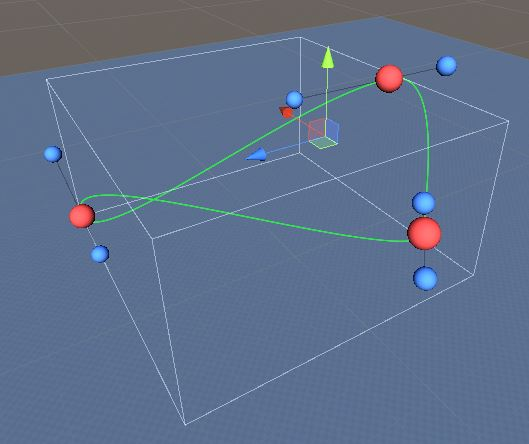
\includegraphics[scale=0.4]{img/contoh-kurva-bezier.JPG}
	\caption{Contoh kurva bezier pada bidang 3 dimensi}
	\label{fig:2.1}
\end{figure}

\textit{Bézier curve} atau kurva bezier adalah kurva parametrik yang banyak digunakan pada bidang grafika komputer serta bidang - bidang lain yang berhubungan. Sifat dari kurva bezier yang parametrik dapat digunakan untuk memodelkan kurva pada 2 atau bahkan 3 dimensi grafika komputer. Selain itu sifat parametrik ini juga membawa sifat lain yang mana menyebabkan kurva bezier memiliki sifat dapat diskalakan sesuai dengan kebutuhan. Kurva bezier memiliki 2 komponen utama, yaitu \textit{control points} atau titik kontrol, serta \textit{anchor points} atau titik jangkar Dengan menentukan lokasi serta orientasi (apabila pada 3 dimensi) dari titik - titik kontrol dan titik jangkar yang digunakan pada kurva bezier, sehingga dapat dimodelkan seluruh jenis kurva dengan mudah, serta pada penerapan di grafika komputer, cukup mudah dalam melakukan operasi transformasi pada titik - titik kontrol untuk mendapatkan jenis kurva yang diinginkan.\cite{cit:9}

\section{\textit{6 Degree of Freedom}}
\vspace{1ex}

\begin{figure}  [!htb]
	        \captionsetup{justification=centering}
	        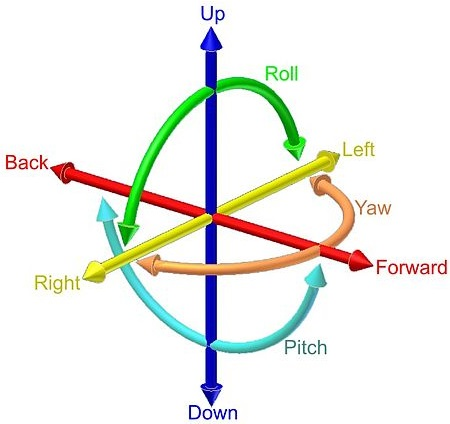
\includegraphics[scale=0.4]{img/6dof.jpg}
	        \caption{\textit{6 Degrees of Freedom - Pitch, Roll,} dan \textit{Yaw}\cite{cit:15}}
	        \label{fig: 3_18}
\end{figure}

\textit{6 Degree of Freedom / DoF}, adalah istilah atau penjelasan dari pergerakan suatu objek pada dimensi spasial ketiga. \textit{DoF} memiliki 3 macam istilah yang perlu di ketahui, Yang pertama \textit{Pitch} ialah merepresentasikan sudut putaran terhadap sumbu \textit{x}, yang kedua \textit{Yaw}, yang merepresentasikan sudut putaran terhadap sumbu \textit{y}, yang ketiga \textit{Roll}, yang merepresentasikan sudut putaran terhadap sumbu \textit{z}.

\section{Kecepatan / \textit{Velocity}}
\vspace{1ex}

\begin{figure}  [!htb]
	        \captionsetup{justification=centering}
	        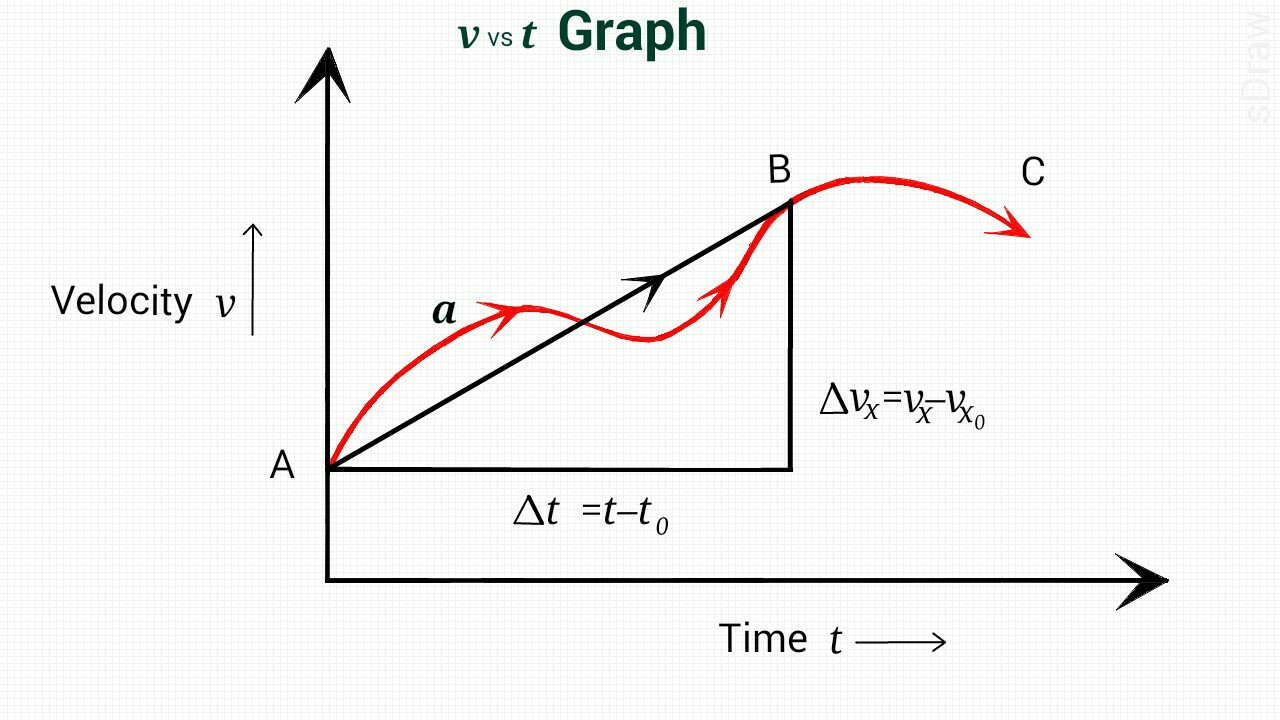
\includegraphics[scale=0.2]{img/velocity.jpg}
        	%\caption{Diagram alur kerja}
        	\caption{Kecepatan}
        	\label{fig: 3_27}
\end{figure}

Kecepatan / \textit{velocity} pada bidang grafika komputer, terdapat 2 jenis yaitu: kecepatan vektor serta besaran kecepatan, kecepatan vektor ialah seberapa unit jauh objek berpindah dalam suatu hitungan waktu terhadap masing - masing sumbu x, y, serta z.

\section{\textit{Colission}}
\vspace{1ex}

Konsep \textit{Collission} pada \textit{Unity Game Engine}, ialah terdapat 2 macam \textit{collider}. \textit{Collider} itu sendiri ialah entitas yang dapat berinteraksi dengan \textit{collider lain}. 2 Macam \textit{collider} adalah \textit{trigger collider} serta \textit{physics collider}. \textit{Physics collider} ialah entitas \textit{collider} yang mensimulasikan hukum fisika dengan akurat, seperti contohnya interaksi roda dengan jalan/tanah, mobil dengan mobil lain, dsb. Sedangkan \textit{Trigger Collider} tidak mensimulasikan hal tersebut, fungsi dari \textit{trigger collider} ialah \textit{unity} dapat mengetahui bahwa suatu entitas \textit{collider} lain telah berinteraksi dengan \textit{trigger collider} tersebut, sehingga dapat melakukan perintah terprogram menggunakan \textit{event system}
\cleardoublepage
\chapter{DESAIN DAN IMPLEMENTASI SISTEM}
\vspace{1ex}

\section*{}
	Penelitian ini dilaksanakan sesuai dengan desain sistem berikut dengan implementasinya. Desain sistem merupakan konsep dari pembuatan dan perancangan infrastruktur kemudian diwujudkan dalam bentuk blok-blok alur yang harus dikerjakan. Pada bagian implementasi merupakan pelaksanaan teknis untuk setiap blok pada desain sistem.
\vspace{1ex}

\section{Cakupan Tugas Akhir}
\vspace{1ex}

	Tugas akhir ini merupakan salah satu bentuk implementasi grafika komputer untuk mensimulasikan pengalaman berkendara yang digabungkan dengan sistem \textit{Microcontroller} untuk pengambilan data, berikut pada Gambar 3.1 adalah cakupan Tugas Akhir dari Desain Sistem.
\begin{figure}  [!htb]
	\captionsetup{justification=centering}
	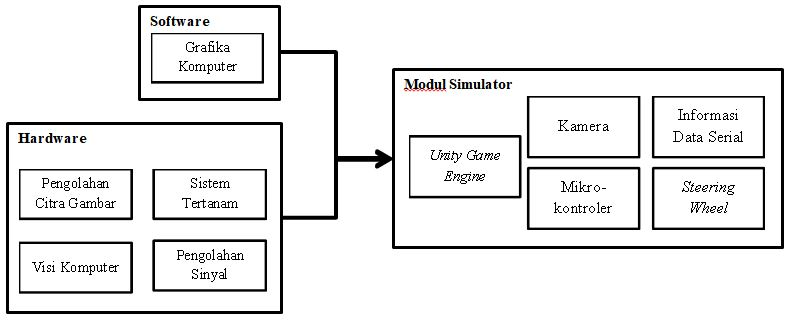
\includegraphics[scale=0.55]{img/cakupanTA.JPG}
	\caption{Blok Diagram Cakupan Disiplin Ilmu Tugas Akhir}
	\label{fig: 3_1}
\end{figure}
\vspace{1ex}
    \subsection{Cakupan \textit{Hardware}}
    Desain sistem secara umum pada gambar \ref{fig: 3_1}, yang mencakup disiplin ilmu perangkat keras atau \textit{hardware}, ialah pengolahan citra gambar, visi komputer, sistem tertanam, serta pengolahan sinyal. Disiplin pengolahan citra gambar didapatkan dari pengambilan citra pengemudi menggunakan kamera, visi komputer didapatkan dari proses \textit{recognition} wajah pengemudi, sistem tertanam atau \textit{embedded system} didapatkan dari komunikasi data - data serial menggunakan Arduino atau Mikroprosesor yang tersambung dengan simulator, kemudian yang terakhir Pengolahan sinyal didapatkan dari pengolahan data - data analog seperti data \textit{Electroencephalography (EEG)} / detak jantung pengemudi, atau data \textit{Electrooculography (EOG)} / data kedipan mata dari pengemudi.
    
    \subsection{Cakupan \textit{Software}}
   Cakupan Tugas Akhir ini pada bagian perangkat lunak atau \textit{software}, lebih ditekankan dalam upaya pembuatan \textit{Simulation Environment} atau Lingkungan Simulasi menggunakan \textit{Unity Game Engine}. \textit{Simulation Environment} dibuat dengan menggunakan disiplin ilmu grafika komputer 3d (3d \textit{Computer Graphics}), serta juga menggunakan proses - proses pengembangan dari \textit{game engine} dan \textit{physics engine} yang lain.
    
    \subsection{\textit{Output yang diharapkan}}
    \textit{Output} atau keluaran yang diharapkan dari tugas akhir ini ialah, dihasilkannya suatu modul simulasi yang terintegrasi lengkap dengan \textit{tools - tools} dan \textit{peripheral} yang yang dapat mensimulasikan suatu pengalaman mengemudi menggunakan suatu \textit{simulator}, serta dapat melakukan proses pengambilan data - data primer yang valid, sehingga dapat diolah untuk proses riset selanjutnya.


\section{Desain Sistem}
\vspace{1ex}
	Pada Tugas Akhir ini, dilakukan penggabungan perangkat lunak berupa \textit{game engine} untuk mensimulasikan proses berkendara, dengan perangkat keras berupa \textit{controller} dari \textit{simulator} dan \textit{Microcontroller} untuk proses pengambilan data. Proses kerja dari sistem ini akan dijelaskan melalui diagram alur pada gambar \ref{fig: 3_2}.
	Selain itu, simulator ini memiliki 2 jenis data yang dapat diukur. Berikut penjelasan 2 macam jenis data tersebut.
\begin{figure}  [!htb]
	\captionsetup{justification=centering}
	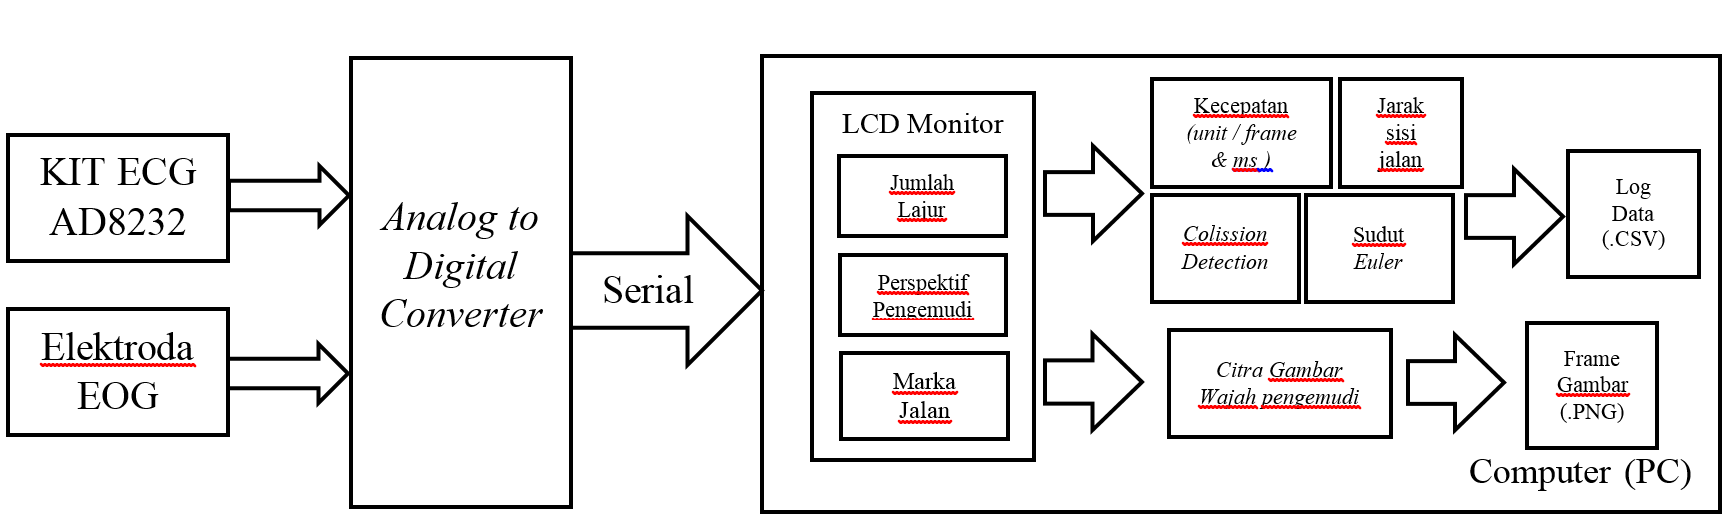
\includegraphics[scale=0.25]{img/desainsistem.PNG}
	%\caption{Diagram alur kerja}
	\caption{Desain umum modul Simulator}
	\label{fig: 3_2}
\end{figure}
\vspace{1ex}

    \subsection{Data - Data Internal Simulator}
    \vspace{1ex}
    Jenis data yang pertama adalah data yang berasal dari dalam modul simulator, yaitu data - data seperti kecepatan mobil, informasi spasial seperti, sudut \textit{euler} \textit{(pitch,yaw,roll)} dan jarak relatif terhadap pinggir jalan, informasi tabrakan / \textit{colission}, serta informasi waktu respon / \textit{response time}. Data - data ini, disebut sebagai data internal, dikarenakan data - data tersebut bisa di ekstraksi langsung dari \textit{game engine}.
    
        \subsubsection{Kecepatan Mobil / \textit{Velocity}}
        
        Pada unity game engine, menggunakan library Unity. Bisa didapatkan secara langsung variabel - variabel yang berhubungan dengan kecepatan. Pada tugas akhir ini, dibutuhkan data kecepatan mobil relatif terhadap dunia atau biasa disebut \textit{global velocity}. Namun selanjutnya, data kecepatan global pun bisa dibagi menjadi 4 macam, yaitu : \textit{velocity} atau kecepatan kearah sumbu \textit{x}, \textit{velocity} atau kecepatan kearah sumbu \textit{y}, serta \textit{velocity} atau kecepatan kearah sumbu \textit{z}, ketiga hal tersebut bisa juga disebut kecepatan vektor \textit{x,y,z}. Dan yang terakhir, adalah \textit{velocity magnitude}, atau tingkat kebesaran suatu kecepatan berupa skalar. Contoh data ini bisa dilihat pada tabel pengujian \ref{tb:4_2}
        
        \subsubsection{Informasi Spasial}
        
        \begin{figure}  [!htb]
	        \captionsetup{justification=centering}
	        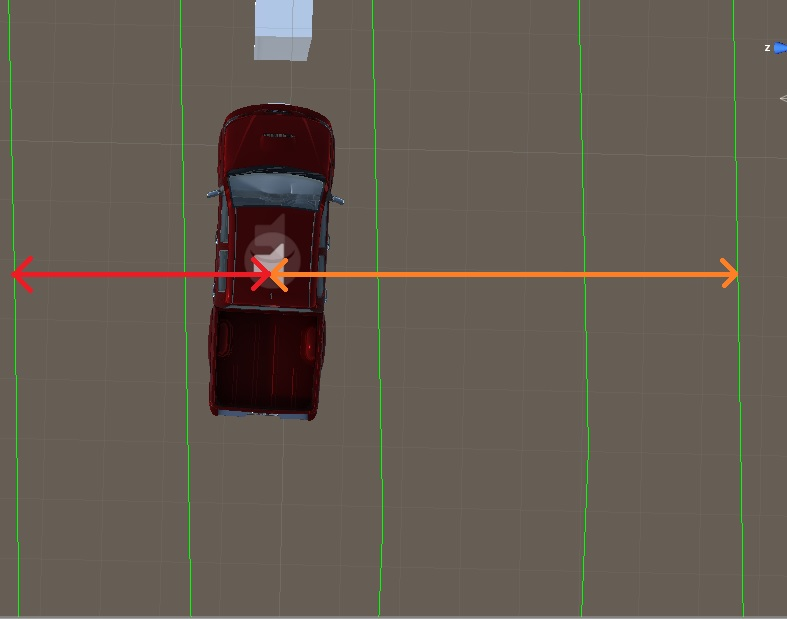
\includegraphics[scale=0.5]{img/relative-dist.jpg}
	        \caption{\textit{Relative Distance} \\ Oranye : Jarak dari \textit{Center of Mass} Mobil ke Batas Pinggir Kanan Jalan \\ Merah : Jarak dari \textit{Center of Mass} Mobil ke Batas Pinggir Kiri Jalan}
	        \label{fig: 3_19}
        \end{figure}
        
        Selain kecepatan, bisa didapatkan pula informasi spasial yang ada pada simulator. Pada tugas akhir ini, informasi spasial simulator adalah sudut euler yang merepresentasikan 6 derajat kebebasan atau biasa disebut \textit{6 Degree of Freedom (DoF))}, yaitu \textit{pitch, yaw,} dan \textit{roll} (gambar \ref{fig: 3_18}). Pada Tugas akhir ini, ketiga macam rotasi atau derajat kebebasan seluruhnya dimanfaatkan pada proses pembuatan desain jalan.
        
        \par Selanjutnya data spasial yang bisa didapatkan ialah posisi relatif kendaraan terhadap pinggir jalan (gambar \ref{fig: 3_19}). Dengan mengukur jarak terdekat dari titik pusat masa atau \textit{Center of Mass} mobil, ke batas pinggir kanan dan batas pinggir kiri jalan, dapat diketahui dimana posisi mobil di suatu lajur tersebut.
        
        \par Dengan menggabungkan dua macam jenis data tersebut, bisa didapatkan informasi yang sangat jelas tentang posisi dan orientasi dari kendaraan pengujian simulator ini. Yang nanti kedepannya sangat dibutuhkan untuk proses riset selanjutnya, yang akan memanfaatkan data - data tersebut.
        
        \subsubsection{Response Time}
        
        \begin{figure}  [!htb]
	        \captionsetup{justification=centering}
	        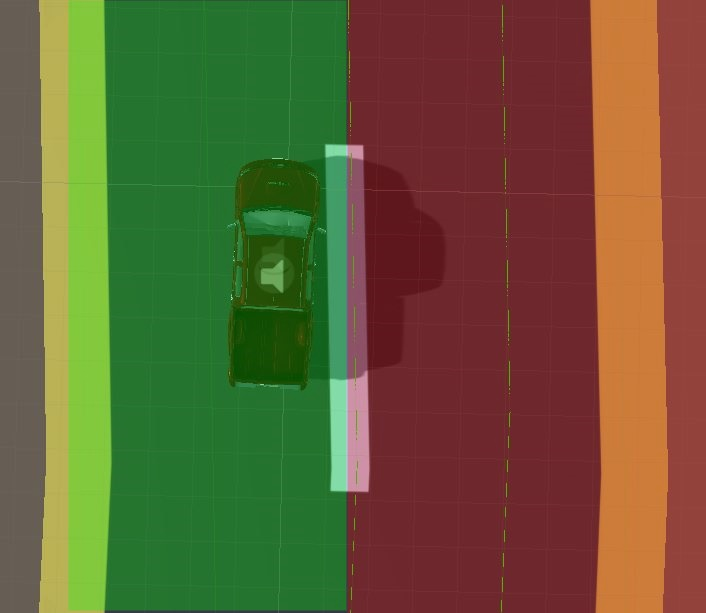
\includegraphics[scale=0.5]{img/jalur-tnp-mobil.JPG}
	        \caption{Response Time - IlustrasiJalur yang diharapkan - Kasus Tidak ada Mobil Lain}
	        \label{fig: 3_20}
        \end{figure}
        
        \begin{figure}  [!htb]
	        \captionsetup{justification=centering}
	        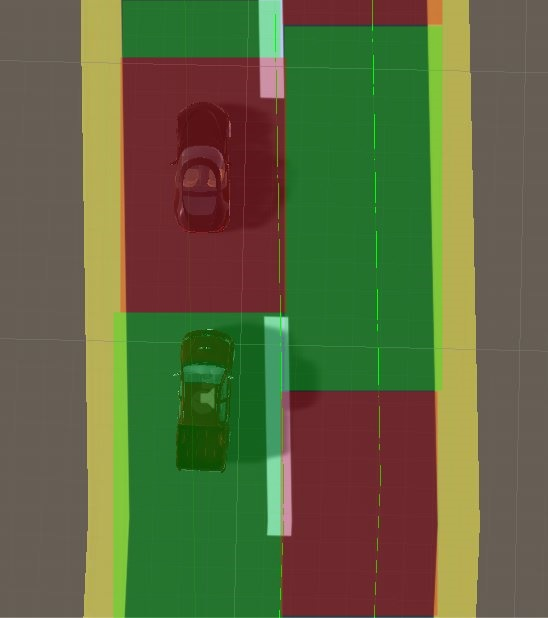
\includegraphics[scale=0.6]{img/jalur-dgn-mobil.JPG}
	        \caption{Response Time - Ilustrasi Jalur yang diharapkan - Kasus terdapat mobil lain}
	        \label{fig: 3_21}
        \end{figure}
        
        \textit{Response time} adalah metode pengukuran tingkat kewaspadaan pengemudi, dengan cara mendeteksi ketika pengemudi keluar dari lajur yang diharapkan. Lajur yang diharapkan disini, yang dimaksud ialah lajur sebelah kiri, dikarenakan desain simulator menggunakan model jalan yang ada di Indonesia. Berikut penjelasan tentang data \textit{Response time} pada gambar \ref{fig: 3_20} dan \ref{fig: 3_21}.
        
        Pada gambar \ref{fig: 3_20}, adalah gambar ilustrasi jalur yang diharapkan, pada kasus dimana tidak ada mobil lain didekat mobil pengujian. Warna hijau menandakan area yang di tandai oleh sistem simulator sebagai jalur yang diharapkan oleh sistem, artinya sistem mendeteksi bahwa mobil pada jalur yang telah sesuai serta pengemudi masih dalam keadaan waspada serta memiliki kontrol terhadap mobil. Apabila sistem mendeteksi mobil memasuki area yang berwarna merah, maka sistem akan melakukan pencatatan data yaitu kapan mobil mulai keluar dari jalur (tanggal dan waktu). Selanjutnya, sistem juga akan melacak mobil apabila mobil telah kembali ke area hijau, yang mana pada saat ini, sistem akan melakukan pencatatan data seberapa lama mobil telah keluar dari area hijau dengan \textit{unit} sekon, yang selanjutnya bisa didapatkan pula, seberapa lama mobil telah keluar dari area hijau dalam \textit{unit} hitungan \textit{frame}, dengan cara mengalikan waktu dalam sekon, dengan \textit{average framerate} dari simulator saat itu.
        
        \par Selanjutnya, pada gambar \ref{fig: 3_21}, adalah ilustrasi kasus dimana terdapat mobil didekat mobil uji, yang menyebabkan berubahnya jalur yang diharapkan. Apabila sistem mendeteksi terdapat mobil lain didekat mobil uji, sistem akan melakukan perubahan jalur yang diharapkan oleh sistem, metode penerapan pendeteksian seperti ini dapat diterapkan dengan banyak cara, salah satunya bisa dilakukan dengan membuat \textit{trigger box colission} disekitar mobil uji, yang mana ukurannya lebih besar dari \textit{bounding box} / ukuran mobil uji. Apabila terdapat suatu objek (seperti mobil lain), yang memasuki \textit{trigger box colission} dari mobil uji, maka bisa dilakukan perubahan pendeteksian jalur. Pada Tugas Akhir ini, digunakan metode ini untuk mendeteksi adanya mobil lain disekitar mobil uji, serta mendeteksi perlu terjadinya perubahan jalur yang diharapkan.
        
        \par Cara lain yang lebih mudah, namun tentunya dengan mengorbankan tingkat keakurasian pendeteksian yaitu adalah, dengan mengukur jarak mobil uji dengan mobil lain. Apabila jarak mobil uji dengan mobil lain ini dibawah nilai threshold, maka bisa dilakukan perubahan jalur yang diharapkan.
        
        \par Selanjutnya perlu digaris bawahi, bahwa sistem deteksi perubahan jalur ini juga sangat berkaitan dengan sistem deteksi terjadinya tabrakan. Sistem pendeteksian dan pencatatan data atau \textit{logging} dari \textit{colission event} ini akan dijelaskan pada subsubbab selanjutnya.
        
        \subsubsection{\textit{Colission Event}}
        
        \begin{figure}  [!htb]
	        \captionsetup{justification=centering}
	        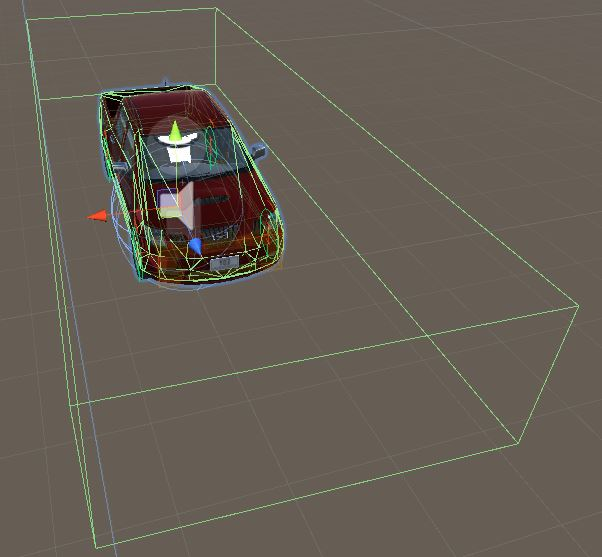
\includegraphics[scale=0.65]{img/colliders.JPG}
	        \caption{2 Macam \textit{Colliders} Mobil - \textit{Box Collider} dan \textit{Mesh Collider}}
	        \label{fig: 3_22}
        \end{figure}
        
        \begin{figure}  [!htb]
	        \captionsetup{justification=centering}
	        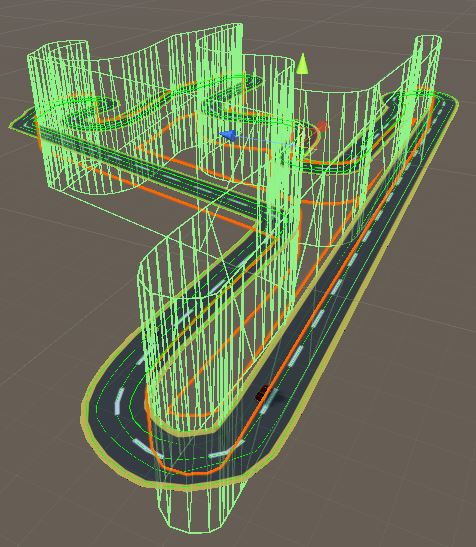
\includegraphics[scale=0.7]{img/boundary-inside.JPG}
	        \caption{\textit{Boundary} dalam sirkuit}
	        \label{fig: 3_23}
        \end{figure}
        
        \begin{figure}  [!htb]
	        \captionsetup{justification=centering}
	        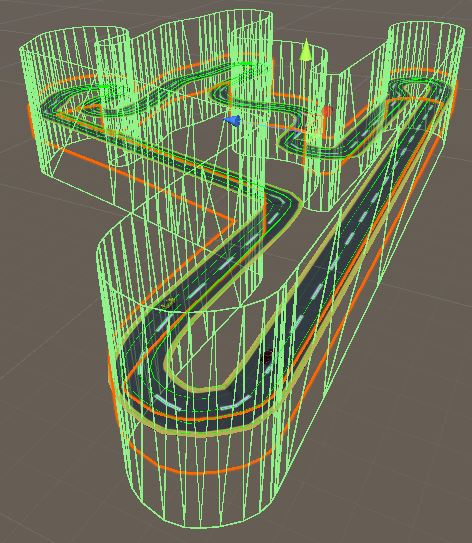
\includegraphics[scale=0.7]{img/boundary-outside.JPG}
	        \caption{\textit{Boundary} luar sirkuit}
	        \label{fig: 3_24}
        \end{figure}
        
         Pada subsubbab sebelumnya telah dijelaskan metode untuk mendeteksi keberadaan mobil lain di dekat mobil uji pada tugas akhir ini, yaitu dengan cara menggunakan \textit{trigger box event}. Pada subsubbab ini, \textit{colission event} yang dimaksud terdapat 2 macam. Yaitu yang pertama adalah, kejadian tabrakan dengan mobil lain, yang kedua kejadian tabrakan dengan pinggir jalan / \textit{boundary}. 
         
         \par Untuk proses pendeteksian tabrakan dengan mobil lain, dapat menggunakan \textit{mesh collider} yang sudah tersedia dengan mobil, untuk mempermudah proses deteksi, serta menyederhanakan \textit{physics interaction} antar mobil. Selain mobil uji, seluruh \textit{mesh collider} dari mobil lain ditentukan sebagai \textit{trigger}. Hal ini untuk menghindari terjadinya interaksi - interaksi yang tidak diinginkan ketika terjadi tabrakan antar mobil. 
         
         \par Dengan menggunakan fungsi \texttt{void onColissionEnter()} dan fungsi \texttt{void onTriggerEnter()} pada unity, dapat dilakukan pengecekan apabila terjadi overlap antar 2 \textit{GameObject} yang ada pada unity. Dengan menentukan \textit{GameObject} mana yang perlu dideteksi, sehingga langkah selanjutnya ialah mencatat data colission kedalam \textit{log file system}, 3 \textit{GameObject} yang perlu dideteksi adalah : \textit{Boundary} Luar / Batas Pinggir Kanan Jalan, \textit{Boundary} Dalam / Batas Pinggir Kiri Jalan, serta Mobil lain.
         
         \par Contoh data yang diambil pada \textit{colission event} bisa dilihat pada tabel \ref{tb:4_5}.
        
    
    \subsection{Data - Data Eksternal Simulator}
    \vspace{1ex}
    
     Selanjutnya Jenis data yang kedua adalah data yang berasal dari luar modul simulator, yaitu data - data seperti sinyal \textit{Electroencephalography (EEG)} / detak jantung pengemudi, dan atau data sinyal \textit{Electrooculography (EOG)} / data kedipan mata dari pengemudi, serta data citra wajah pengemudi menggunakan kamera. Data - data tersebut diatas, dikatakan sebagai data eksternal dikarenakan data - data tersebut didapatkan dari peralatan \textit{peripheral} yang dipasang pada modul simulator. Berhubung data EEG dan EOG merupakan data sinyal analog, maka diperlukannya suatu \textit{Analog to Digital Converter} atau ADC, supaya data bisa di rekam dalam \textit{log file}.
     Tentunya, perlu diperhatikan juga sampling rate dari ADC ini, sehingga bisa relevan dan dapat disesuaikan dengan data - data yang lain.
     
        \subsubsection{\textit{Serial Communication} Melalui \textit{port} COM}
        Pada tugas akhir ini, \textit{serial communication} melalui \textit{port} COM, dilakukan menggunakan \textit{Python}. Diagram \textit{flow chart} dari proses komunikasi data serial arduino ke PC, bisa di lihat pada gambar \ref{fig: 3_25}.
        \par Proses dari modul pembacaan data serial dimulai dengan pembuatan \textit{file} dengan nama tanggal dijalankannya modul tersebut. Hal ini dilakukan untuk mengetahui kapan waktu dan tanggal modul pembacaan dijalankan. Selain itu, hal ini memastikan bahwasanya file - file dapat dipisahkan atau disortir berdasarkan waktu dan tanggal, yang artinya data - data yang dicatat, tidak akan bercampur aduk dengan data - data percobaan yang sebelumnya.
        \par Dengan mengasumsikan bahwa arduino akan melakukan pengiriman data, \textit{python} akan terus membaca data dari arduino, dengan maksimum \textit{baudrate} yang telah ditentukan. Kemudian, setelah proses pembacaan dilakukan, akan dilakukan proses \textit{decode}. Proses \textit{Decode} ialah proses dimana \textit{python} akan melakukan konversi data biner, menjadi data - data diskrit \textit{integer} / bilangan bulat, yang kemudian hasil dari proses \textit{decode}, akan dilakukan proses append pada \textit{file} yang telah dibuat sebelumnya. 
        \par Informasi lebih jelas tentang proses \textit{append file} dan \textit{log file system} akan dijelaskan lebih lanjut pada sub-bab \ref{logfilesystem}
        
        \subsubsection{Citra Wajah Pengemudi / \textit{Webcam}}
        Pada \textit{Unity Game Engine}, sistem mensupport pembacaan informasi kamera webcam sebagai salah satu bagian dari \textit{library mobile camera information}, yang artinya adalah, apabila platform dari simulator menggunakan PC dengan OS \textit{Windows}, dan terdapat \textit{peripheral Webcam} yang terpasang, Unity dapat mendeteksi \textit{webcam} tersebut sebagai \textit{Imaging Device}.
        \par Sebagai \textit{Imaging Device}, data yang diperoleh unity dari \textit{webcam} ditangkap sebagai \textit{texture information}, atau informasi texture dari suatu \textit{GameObject}.
        
        \begin{figure}  [!htb]
	        \captionsetup{justification=centering}
	        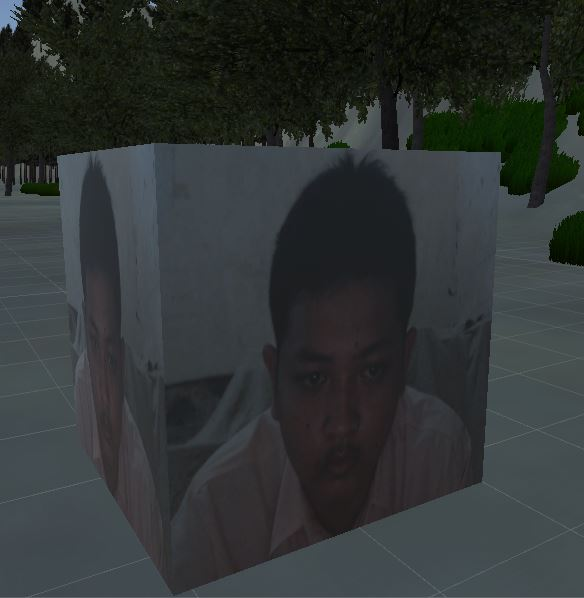
\includegraphics[scale=0.62]{img/webcam-texture.JPG}
	        \caption{Kubus yang memiliki \textit{texture information} dari \textit{Webcam / Imaging Device}}
	        \label{fig: 3_26}
        \end{figure}
        
       Dikarenakan informasi yang ditangkap oleh unity merupakan suatu \textit{texture}, maka \textit{texture} tersebut bisa di pasangkan ke suatu \textit{GameObject}, agar memiliki tampilan dari \textit{webcam}.  Bisa dilihat, pada gambar \ref{fig: 3_26}, ketika informasi webcam di pasangkan dengan kubus.
       \par Namun pada tugas akhir ini, yang dibutuhkan bukanlah informasi \textit{texture} yang bisa digunakan oleh game ini. Yang dibutuhkan adalah \textit{frame - frame} / gambar wajah dengan \textit{timestamp} yang sesuai. Maka langkah selanjutnya adalah mengekstrak informasi \textit{texture} tersebut keluar dari unity. Hal ini mudah dilakukan dengan melakukan fungsi \textit{encoding} ke tipe \textit{file} yang berekstensi \textit{PNG}. Setelah encoding dilakukan, \textit{file stream} akan menuliskan data hasil \textit{encoding} menjadi suatu gambar lengkap dengan \textit{timestamp} nya.
       \par Hasil pengujian pengambilan data citra wajah pengemudi menjadi frame - frame yang telah di \textit{encode} menjadi PNG bisa di lihat pada gambar \ref{fig:4.2}
    
\section{Desain Lajur Simulator}
\vspace{1ex}

    \par Pada tugas akhir ini, terdapat 4 macam lajur yang dapat dipilih oleh pengemudi. 4 Macam lajur tersebut berfungsi sebagai basis riset untuk mengeliminasi terjadinya bias atau pengaruh yang dihasilkan oleh perbedaan jumlah lajur yang digunakan.
    
\begin{figure}  [!htb]
	\captionsetup{justification=centering}
	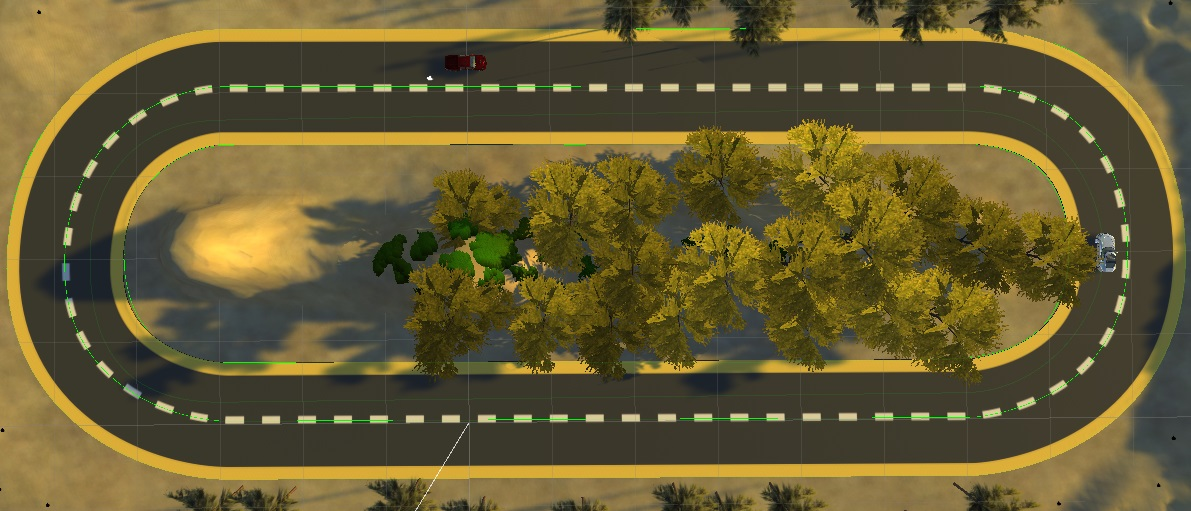
\includegraphics[scale=0.31]{img/2lj_short_oh.jpg}
	\caption{Desain sirkuit 2 lajur dengan jarak yang pendek dan kompleksitas yang rendah}
	\label{fig: 3_3}
\end{figure}
\vspace{1ex}

\begin{figure}  [!htb]
	\captionsetup{justification=centering}
	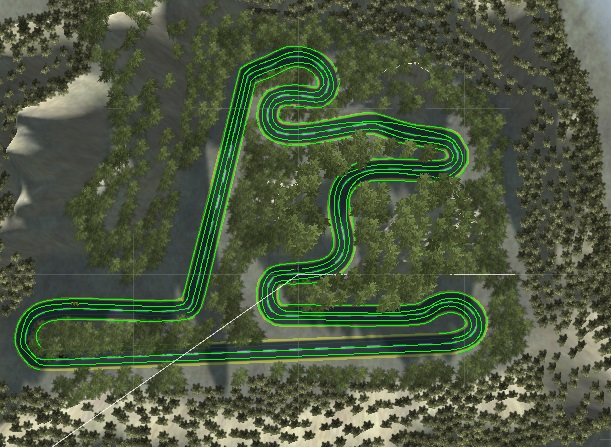
\includegraphics[scale=0.53]{img/2lj_long_oh.jpg}
	\caption{Desain sirkuit 2 lajur dengan jarak yang panjang dan kompleksitas yang tinggi}
	\label{fig: 3_4}
\end{figure}
\vspace{1ex}

\begin{figure}  [!htb]
	\captionsetup{justification=centering}
	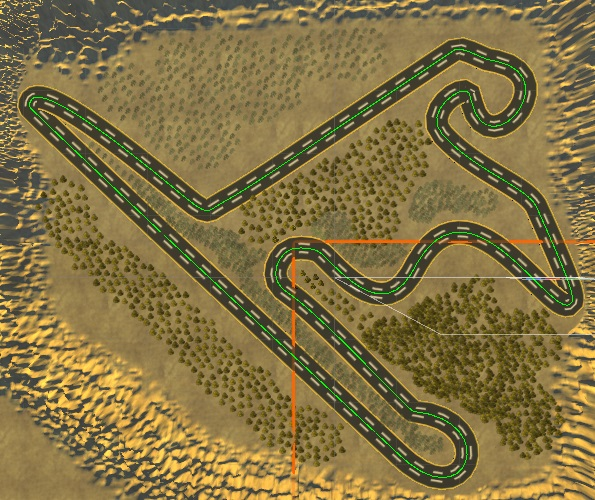
\includegraphics[scale=0.53]{img/3lj_oh.jpg}
	\caption{Desain sirkuit 3 lajur}
	\label{fig: 3_5}
\end{figure}
\vspace{1ex}

\begin{figure}  [!htb]
	\captionsetup{justification=centering}
	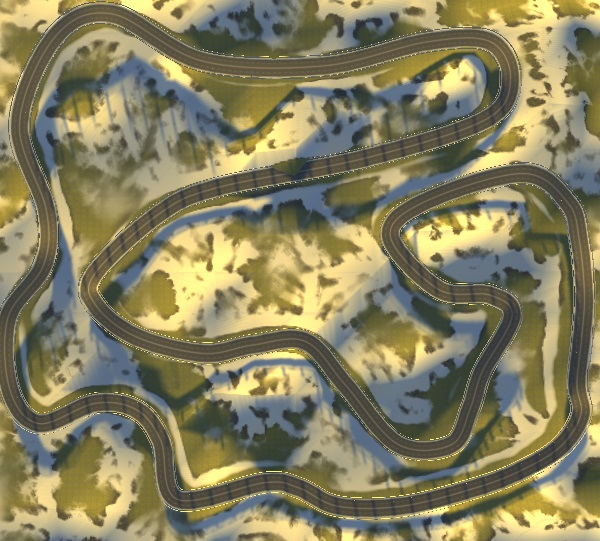
\includegraphics[scale=0.53]{img/4lj_oh.jpg}
	\caption{Desain sirkuit 4 lajur}
	\label{fig: 3_6}
\end{figure}
\vspace{1ex}

    \par Berikut pada Gambar \ref{fig: 3_3}, \ref{fig: 3_4}, \ref{fig: 3_5}, dan \ref{fig: 3_6}, adalah tampak atas dari desain - desain lajur yang digunakan pada simulator ini, seluruh lajur didesain dengan bentuk \textit{closed-loop circuit}. Hal ini bertujuan agar mengurangi ukuran aset jalan yang akan digunakan. Selain itu desain seperti ini dapat berdampak pada durasi pengambilan data, desain sirkuit yang \textit{closed-loop} memungkinkan kegiatan proses pengambilan data supaya tidak bergantung pada panjang jalan yang digunakan.
    \par Tabel \ref{tb:3_1} adalah detil informasi dari desain jalan / sirkuit yang dibuat pada simulator ini. 
    
\begin{table}[]
\caption{Tabel Informasi Sirkuit Jalan}
\label{tb:3_1}
\begin{tabular}{|c|c|c|c|c|c|}
\hline
\multirow{2}{*}{No.} & \multirow{2}{*}{\begin{tabular}[c]{@{}c@{}}Jumlah Lajur\\ (Unit)\end{tabular}} & \multirow{2}{*}{\begin{tabular}[c]{@{}c@{}}Jarak\\ (Unit)\end{tabular}} & \multirow{2}{*}{\begin{tabular}[c]{@{}c@{}}Lebar\\ (Unit)\end{tabular}} & \multicolumn{2}{c|}{\begin{tabular}[c]{@{}c@{}}Kompleksitas\\ (Tampak Atas)\end{tabular}} \\ \cline{5-6} 
                     &                                                                                &                                                                         &                                                                               & \textit{CW Curve}                           & \textit{CCW Curve}                          \\ \hline
1                    & 2                                                                              & 43,145                                                                  & 12                                                                            & 4                                           & 0                                           \\ \hline
2                    & 2                                                                              & 260.226                                                                 & 12                                                                            & 6                                           & 10                                          \\ \hline
3                    & 3                                                                              & \multicolumn{1}{l|}{260.226}                                            & 16                                                                            & 6                                           & 10                                          \\ \hline
4                    & 4                                                                              & 411.346                                                                 & 20                                                                            & 11                                          & 12                                          \\ \hline
\end{tabular}
\end{table}
    
\section{Desain \textit{Behaviour} dari Kendaraan Lain}
\vspace{1ex}

    \par Pada Tugas akhir ini, Desain dari \textit{AI Behavior} kendaraan lain cukup mengikuti lajur sirkuit sesuai dengan jalur yang telah didefinisikan oleh \textit{Bézier curve}, kemudian pada script \textit{follower} yang ada di unity, dikarenakan desain lajur yang \textit{closed-loop}, perlu di definisikan arah dari kendaraan tersebut, dilihat dari tampak atas, apakah kendaraan memiliki \textit{clockwise path} atau \textit{counter-clockwise path}.
    \par Selain arah dari kendaraan, diperlukannya pendefinisian kecepatan kendaraan tersebut, pada Tugas Akhir ini kecepatan kendaraan ditentukan dengan randomisasi dalam suatu rentang tiap kali simulator dijalankan.
    \par Informasi detil dari desain AI kendaraan lain di \textit{unity}, dapat dilihat pada tabel \ref{tb:3_2}

\begin{table}[]
\caption{Tabel Informasi AI Tiap - Tiap Tipe Lajur}
\label{tb:3_2}
\begin{tabular}{|c|c|c|c|c|c|c|}
\hline
\multirow{2}{*}{No.} & \multirow{2}{*}{Lajur} & \multirow{2}{*}{\begin{tabular}[c]{@{}c@{}}Jumlah\\ Mobil\end{tabular}} & \multicolumn{2}{c|}{\textit{AI Rotation}}             & \multicolumn{2}{c|}{\textit{\begin{tabular}[c]{@{}c@{}}Velocity\\ (Unit/Frame)\end{tabular}}} \\ \cline{4-7} 
                     &                        &                                                                         & \textit{CW}               & \textit{CCW}              & \textit{Min}                                  & \textit{Max}                                  \\ \hline
1                    & \textit{2 (Short)}     & 1                                                                       & \xmark     & \checkmark & 5.0f                                          & 15.0f                                         \\ \hline
2                    & \textit{2 (Long)}      & 2                                                                       & \checkmark & \checkmark & 0.1f                                          & 0.9f                                          \\ \hline
3                    & 3                      & 3                                                                       & \checkmark & \checkmark & 0.1f                                          & 0.9f                                          \\ \hline
4                    & 4                      & 4                                                                       & \checkmark & \checkmark & 0.01f                                         & 0.1f                                          \\ \hline
\end{tabular}
\end{table}

\section{Alur Kerja}
\vspace{1ex}

Pembuatan tugas akhir ini dibagi menjadi beberapa tahapan, yaitu:
    \begin{enumerate}[nolistsep]
	
	\item \nohyphens{Pembuatan Simulasi Menggunakan \textit{Unity Game Engine}}
	\item Pengaturan dan Konfigurasi \textit{Steering Wheel Controller} 
	\item Pembuatan Modul Pengambilan Data dengan \textit{Microcontroller}
	\item Penggabungan Seluruh Sistem Menjadi Satu Modul
	
	\end{enumerate}

\section{Pembuatan Simulasi Menggunakan \textit{Unity Game Engine}}
\vspace{1ex}
   Pada Tugas Akhir ini, proses pembuatan simulasi menggunakan \textit{Unity Game Engine}. Namun tidak hanya menggunakan \textit{Unity Game Engine} saja, tentunya selain memanfaatkan \textit{unity editor}, juga diperlukan \textit{source code editor}, pada tugas akhir ini menggunakan \textit{Visual Studio 2017}. Selain itu terdapat \textit{tools - tools} lain di luar \textit{unity} yang dapat mempermudah proses pembuatan Simulator ini.
	
	\subsection{Pembuatan Sirkuit Jalan}
	\vspace{1ex}
	
	\begin{figure} [!htb]
	    \captionsetup{justification=centering}
	    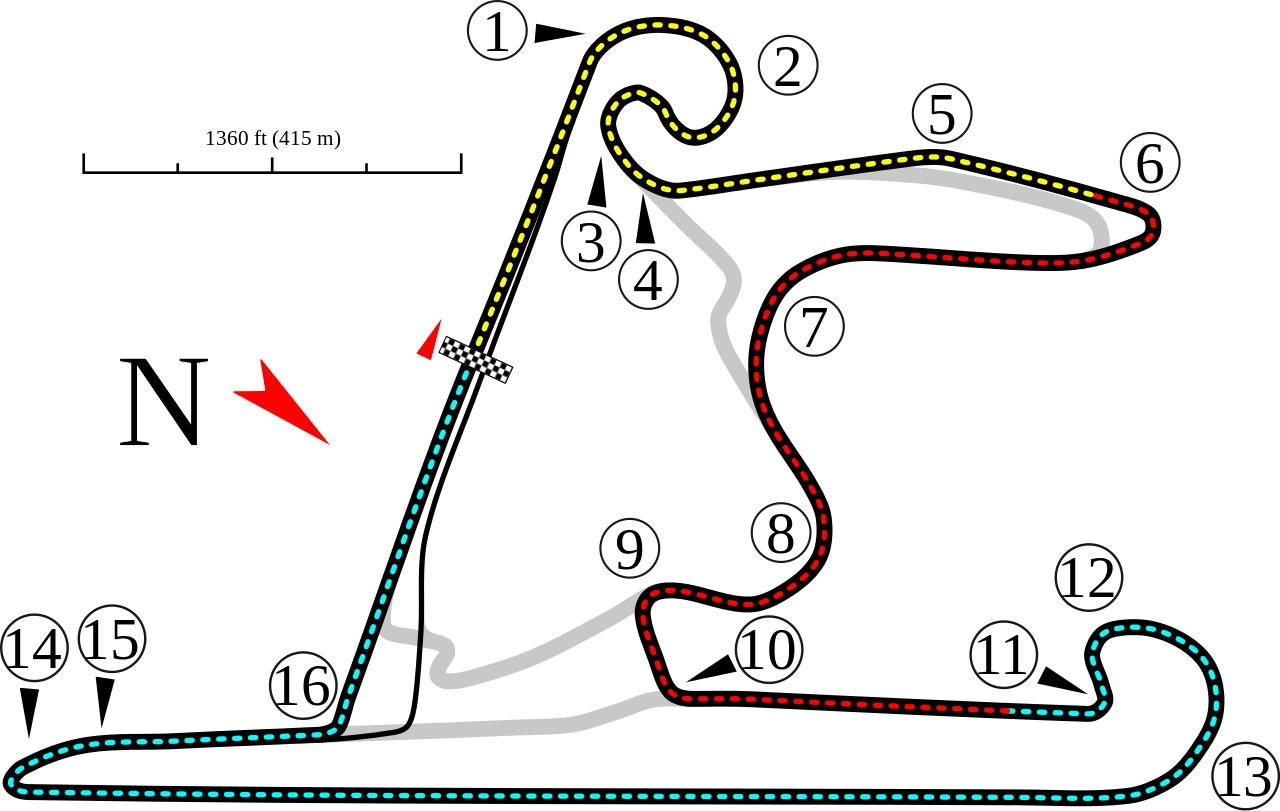
\includegraphics[scale=0.25]{img/shanghai-ic.png}
	    \caption{\textit{Shanghai International Circuit\cite{cit:14}}}
	    \label{fig: 3_10}
    \end{figure}
	
	\begin{figure} [!htb]
	    \captionsetup{justification=centering}
	    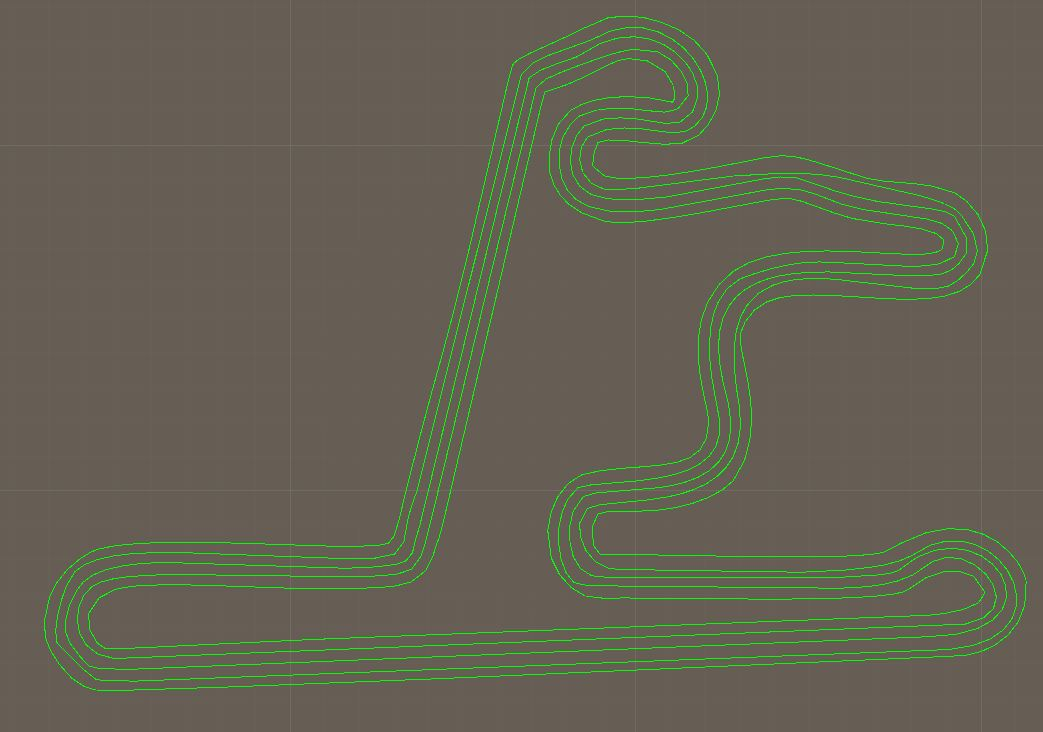
\includegraphics[scale=0.36]{img/bezier-curve-jalan.JPG}
	    \caption{5 Macam \textit{Bézier curve} sirkuit (dari kiri ke kanan) : batas kiri jalan, \textit{Vehicle AI Path - Counterclock Wise}, tengah lajur / marka jalan, \textit{Vehicle AI Path - Clock Wise}, serta batas kanan jalan }
	    \label{fig: 3_9}
    \end{figure}
	
	Proses pembuatan sirkuit jalan adalah proses yang paling memakan waktu pada tugas akhir ini. Yang pertama perlu dilakukan adalah mendefinisikan \textit{path} jalan menggunakan \textit{Bézier curve}, atau jalur yang akan digunakan sebagai \textit{base} dari \textit{3d mesh} jalan atau lajur itu sendiri, salah satu contohnya adalah pada gambar \ref{fig: 3_9}, bisa dilihat terdapat 5 macam kurva bezier yang dapat ditemukan. Semua 5 kurva tersebut dibutuhkan untuk proses kalkulasi informasi jarak serta informasi \textit{colission} yang nantinya akan disimpan kedalam \textit{log file}.
	\par Menggunakan \textit{Shanghai International Circuit} dari \textit{Formula 1}, sebagai referensi bentuk dari sirkuit, diperlukannya penyesuaian tingkat kelengkungan dari belokan yang ada pada sirkuit referensi. Untuk menghindari \textit{mesh overlap}, maka tiap - tiap tikungan yang tajam, perlu diperhalus sedemikian hingga \textit{mesh overlap} agar tidak terjadi. Namun tidak terlalu dikurangi sehingga pengemudi tetap waspada terhadap tikungan tersebut, serta supaya pengemudi mengurangi kecepatan sebelum melakukan belokan tersebut.
	\par Hal ini penting, dikarenakan pada saat proses pengujian berjalan, mobil tidak diharapkan untuk keluar dari lajur pengujian.
	    
	    \subsubsection{\textit{Editing Tools : Path Creator}}
	    \vspace{1ex}
	    
	    \begin{figure} [!htb]
	        \captionsetup{justification=centering}
	        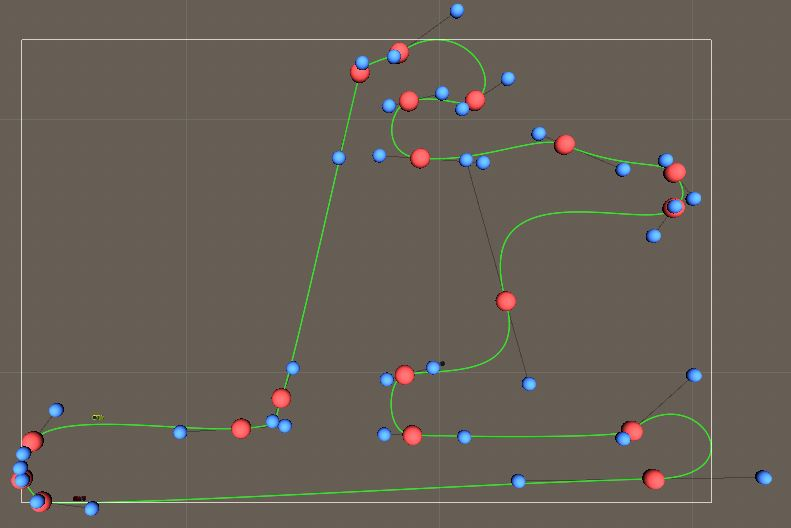
\includegraphics[scale=0.47]{img/bezier-curve-cp.JPG}
	        \caption{\textit{Bézier curve} tampak atas, merah : \textit{anchor points}, biru : \textit{control points}}
	        \label{fig: 3_11}
        \end{figure}
        
        \begin{figure} [!htb]
	        \captionsetup{justification=centering}
	        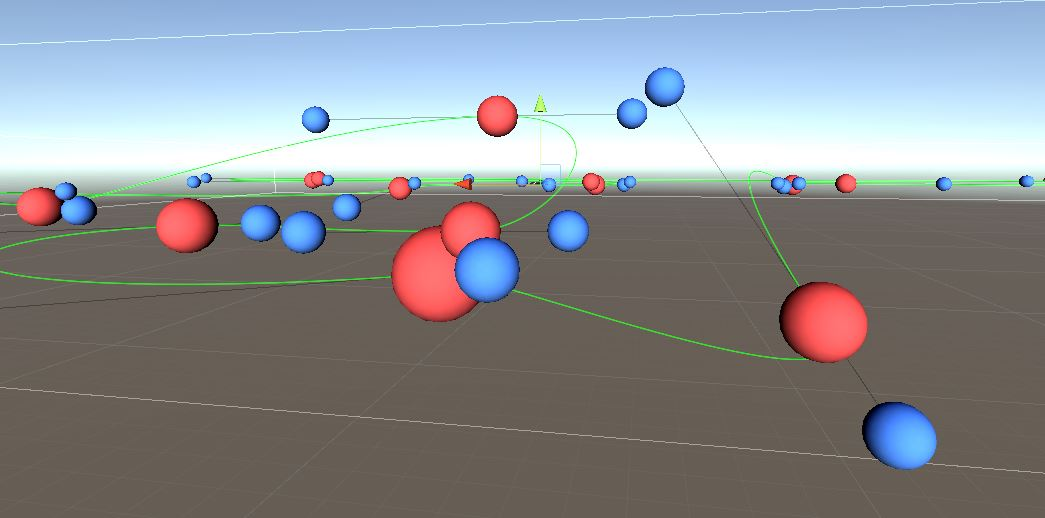
\includegraphics[scale=0.35]{img/bezier-curve-cp2.JPG}
	        \caption{\textit{Bézier curve} pada \textit{3d plane}}
	        \label{fig: 3_12}
        \end{figure}
	    
	    Untuk memudahkan proses pembuatan \textit{Bézier curve}, pada unity. Penulis menggunakan \textit{tools} yang tersedia di unity yang berfungsi untuk mempermudah kalkulasi matematis serta proses \textit{scripting} yang ada pada unity untuk menghasilkan kurva tersebut. Tools tersebut ialah \textit{Path Creator} oleh Sebastian Lague, Path Creator ini dipilih dikarenakan, memudahkan dalam proses manipulasi kurva \textit{Bézier}. Dikarenakan pada \textit{unity} tidak mensupport kurva \textit{Bézier} secara natif, maka biasanya para \textit{game developer}, membuat \textit{script} mereka masing - masing untuk membuat kurva \textit{Bézier}, dengan melakukan kalkulasi persamaan matematis pada script mereka tersebut, kemudian diperlukannya manipulasi titik - titik kontrol sesuai dengan \textit{script} tersebut.
	    \par Namun \textit{Path Creator} memungkinkan penulis untuk melewati proses kalkulasi matematis serta pendefinisian titik - titik kontrol, langsung ke proses manipulasi \textit{drag and drop} titik - titik kontrol, pada \textit{Unity Editor}.
	    \par Pada gambar \ref{fig: 3_11} dan \ref{fig: 3_12}, bisa dilihat titik - titik yang dapat dimanipulasi menggunakan \textit{Path Creator}. Warna merah menunjukkan \textit{anchor points}, yang artinya titik tersebut merupakan titik - titik statis pada suatu persamaan kurva, dengan memanipulasi lokasi dari \textit{anchor points} pada 3 dimensi, dapat didapatkan bentuk \textit{approximation} dari target sirkuit diinginkan. Tentunya, semakin banyak \textit{anchor points} yang digunakan, semakin akurat pula \textit{approximation} jalan yang dibuat. Namun tentunya, kurva jalan menjadi lebih kompleks serta lebih sulit untuk dimanipulasi.
	    \par Kemudian, warna biru menunjukkan \textit{control points}, \textit{control points} ini menentukan lengkungan yang diharapkan diantara tiap - tiap \textit{anchor points}, tentunya agar didapatkankannya lengkungan yang sesuai dengan belokan yang ada pada sirkuit referensi, titik - titik inilah yang akan dapat dimanipulasi.
	    
	    \subsubsection{\textit{Plane Projection} serta \textit{Normal Vector}}
        
        Pada Tugas Akhir ini, informasi tentang \textit{plane projection} yang ada pada kurva \textit{Bézier} sangat penting. Hal ini dapat menunjukkan informasi tentang kekasaran medan atau \textit{level} ketinggian dari suatu daerah pada \textit{terrain} yang ada pada jalan.
        
        \par Pada Tugas akhir ini, jalan yang memiliki 2 dan 3 lajur, memiliki \textit{plane projection} terhadap \textit{XZ Plane}, artinya medan yang ada pada kedua macam jumlah lajur tersebut memiliki kedataran yang seragam, tidak memiliki tanjakan ataupun turunan. 
        
        \par Sedangkan, pada jalan yang memiliki 4 lajur, dengan memanfaatkan semua sumbu \textit{XYZ} maka dapat dihasilkan jalur yang memiliki tanjakan dan turunan.
        
        \begin{figure} [!htb]
	        \captionsetup{justification=centering}
	        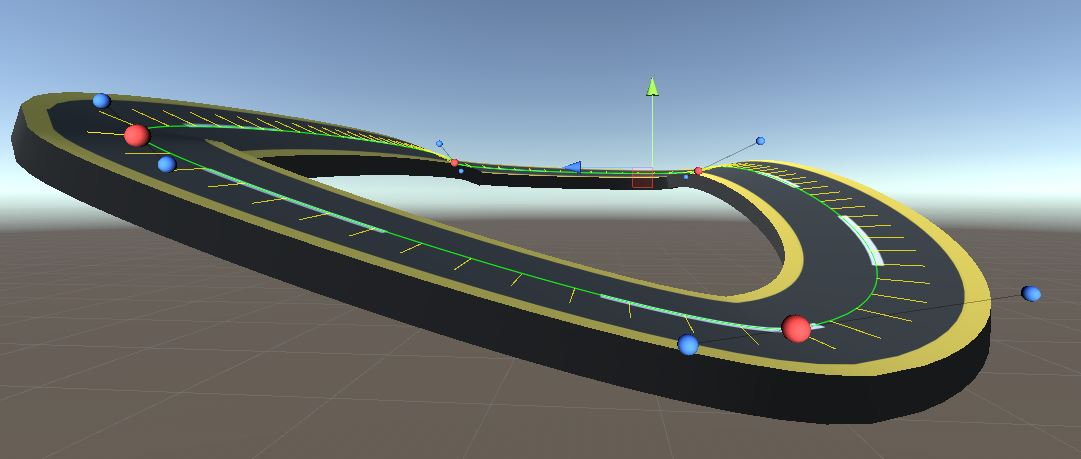
\includegraphics[scale=0.35]{img/pp1.JPG}
	        \caption{\textit{Normal Force} Jalan (\textit{Yaw} 0 Derajat)}
	        \label{fig: 3_13}
        \end{figure}
        
        \begin{figure} [!htb]
	        \captionsetup{justification=centering}
	        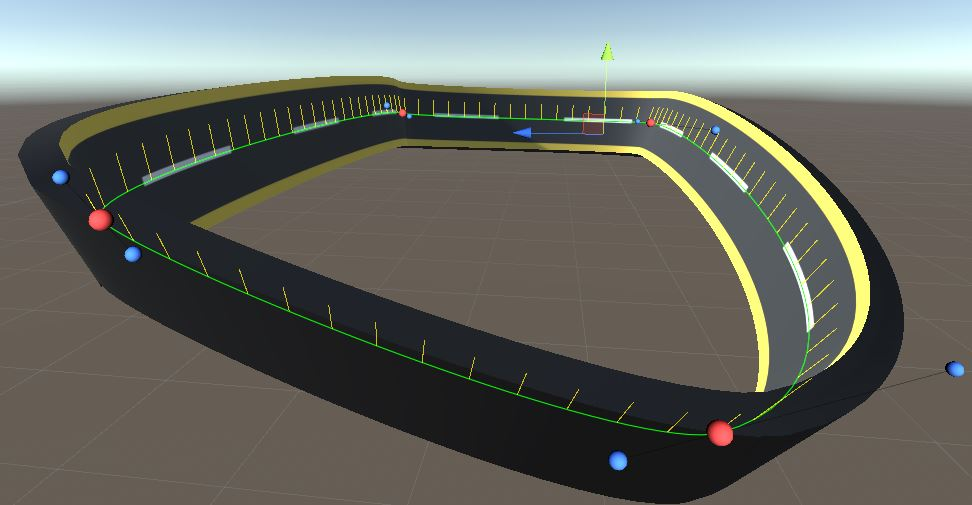
\includegraphics[scale=0.35]{img/pp2.JPG}
	        \caption{\textit{Normal Force} Jalan (\textit{Yaw} 60 Derajat)}
	        \label{fig: 3_14}
        \end{figure}
        
        Kemudian selanjutnya adalah, penentuan \textit{normal force}. Pada \textit{path creator}, parameter yang dapat dikontrol adalah \textit{global angle}, dari normal force tersebut. Hal ini menentukan sudut rotasi / \textit{yaw}, dari jalan yang dibuat pada path yang ditentukan.
        \par Berikut pada gambar \ref{fig: 3_13} dan gambar \ref{fig: 3_14}, perbandingan efek dari \textit{normal force} yang ada di jalan. Hal ini penting diperhatikan untuk proses desain serta pembuatan jalan, yang memanfaatkan seluruh 6 derajat kebebasan \textit{(Degree of Freedom)}, \textit{pitch, yaw,} dan \textit{roll}
	
	\subsection{Pembuatan \textit{Terrain}}
	\vspace{1ex}
	
	Medan atau \textit{terrain}, merupakan kanvas kosong dari sebuah \textit{scene}, yang dapat diisi dengan berbagai macam objek - objek estetis untuk meningkatkan realisme dan imersivitas pada proses simulasi. Pada tugas akhir ini medan yang dibuat pada tiap lajur tidak terlalu berpengaruh terhadap proses pengambilan data itu tersendiri, namun merupakan salah satu \textit{design choice} atau proses pemilihan desain agar meningkatkan kualitas dari \textit{user experience}.
	
	\par Setelah proses pembuatan jalan selesai, untuk meningkatkan estetika, diperlukannya \textit{terrain} yang mengelilingi jalan. Pada \textit{Unity,} objek - objek \textit{non-colission} dapat ditaruh untuk meningkatkan estetika tersebut. Seperti contohnya, pohon - pohon dan semak - semak atau rerumputan. Selain itu, dapat diterapkan perubahan kontur dari \textit{terrain}. Seperti contohnya dapat diterapkan proses peninggian sebagian dari \textit{terrain} untuk menghasilkan bukit, atau bahkan sebaliknya, proses penurunan dari sebagian \textit{terrain} dapat menghasilkan lembah.
	
    Selain itu, pada \textit{unity} dapat ditambahkannya tekstur pada \textit{terrain}. Tekstur disini yang dimaksud ialah, warna atau gambar yang dapat diterapkan pada \textit{terrain} agar menghasilkan corak pada \textit{terrain}. Seperti contohnya tekstur dari tanah coklat, atau tekstur warna pasir kuning, dan sebagainya.
    
    \begin{figure} [!htb]
	    \captionsetup{justification=centering}
	    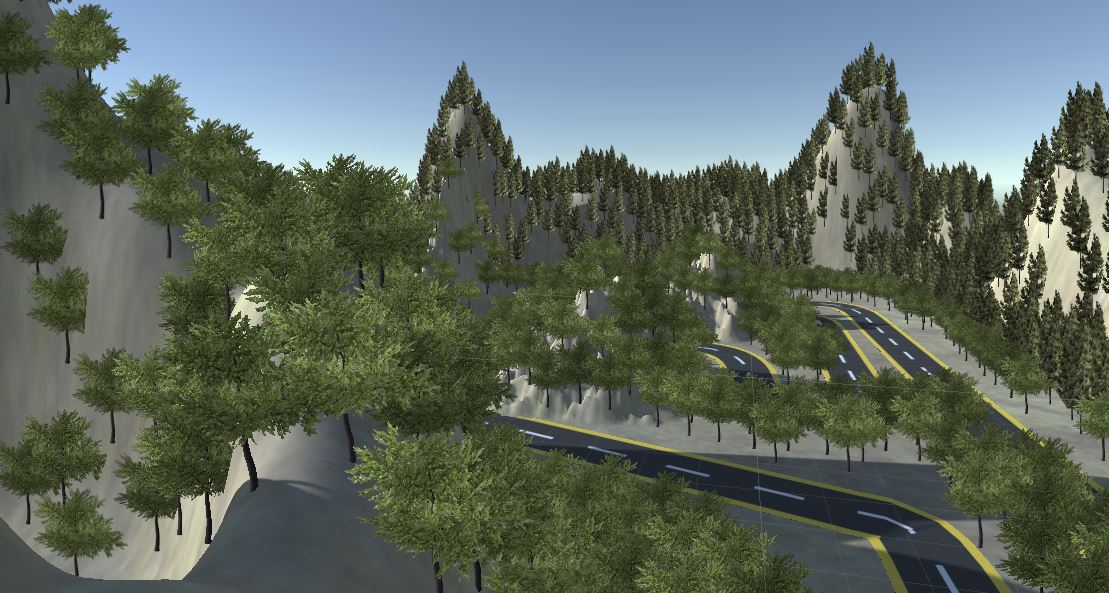
\includegraphics[scale=0.35]{img/terrain.JPG}
	    \caption{\textit{Terrain} setelah ditambahkan bukit, dan pepohonan}
	    \label{fig: 3_17}
    \end{figure}
    
    Selanjutnya, perlu di garis bawahi juga, pada Tugas Akhir ini, salah satu \textit{design choice} merupakan jalan berbentuk sirkuit, maka dari itu terrain, untuk mengakomodasi hal tersebut di terapkan bukit yang mengelilingi sirkuit jalan, untuk memberikan kesan bahwasanya mobil tidak dapat keluar dari lajur.
    
    \subsection{\textit{Menu} dan \textit{User Interface}}
    
    Proses pembuatan Menu dibutuhkan untuk memudahkan pemilihan jumlah lajur nanti setelah simulator menjalani proses \textit{build}. Menu disini dibutuhkan agar tidak terlalu kompleks, namun cukup agar menu dapat menjelaskan serta merepresentasikan tampilan atau tombol yang ditekan. Pemilihan yang intuitif serta fungsionalitas yang berjalan sudah cukup untuk proses ketika di menu.
    \par Perlu diperhatikan juga, dapat diterapkan pula \textit{asynchronous loading}, pada menu ini. Artinya, \textit{scene} atau jenis lajur yang dipilih, akan di muat sebelum tombol ditekan. Supaya proses \textit{loading} akan menjadi lebih cepat.
    
    \begin{figure} [!htb]
	    \captionsetup{justification=centering}
	    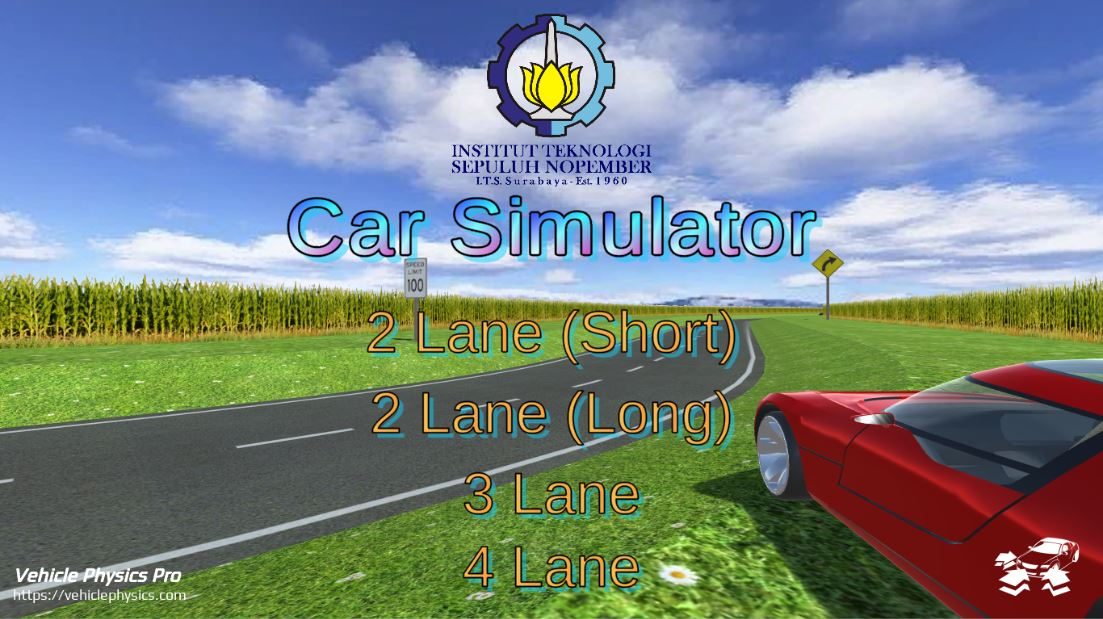
\includegraphics[scale=0.35]{img/menuUI.JPG}
	    \caption{\textit{User Interface} dari Menu}
	    \label{fig: 3_15}
    \end{figure}
    
    Gambar \ref{fig: 3_16} adalah, gambar yang menunjukkan hasil menu yang dibuat. Terdapat 4 tombol yang bisa ditekan, tiap - tiap tombol memiliki penjelasan \textit{text} yang jelas, yaitu merepresentasikan tombol yang akan membawa \textit{user} menuju \textit{scene} atau lajur yang sesuai dengan text tersebut, seperti 2 lajur pendek, 2 lajur panjang, 3 lajur, serta 4 lajur. Selain itu, dipasang pula \textit{background canvas} serta logo ITS pada \textit{User Interface} Menu.
    
    \subsection{\textit{Log File System} dan \textit{Kalkulasi Data}} 
    \label{logfilesystem}
    
    \textit{Log File System} adalah salah satu komponen penting dari Tugas Akhir ini, agar didapatkan suatu \textit{Log File System}, beberapa macam komponen dibutuhkan dari sistem ini (gambar \ref{fig: 3_15}).
    
    \begin{figure} [!htb]
	    \captionsetup{justification=centering}
	    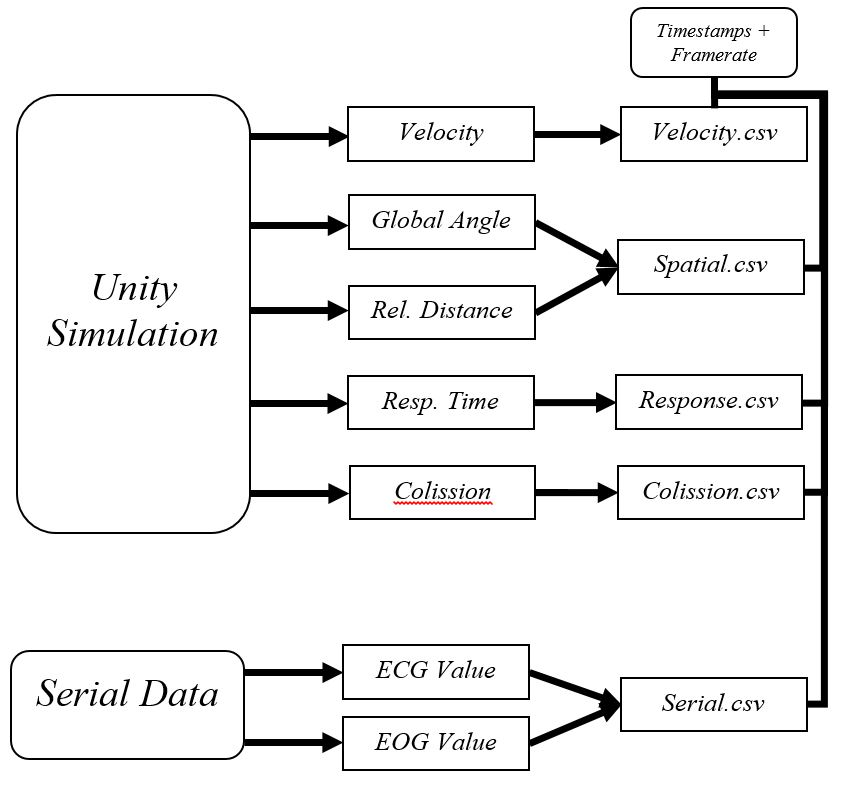
\includegraphics[scale=0.5]{img/logfile.JPG}
	    \caption{Diagram \textit{Log File System}, proses ekstraksi data, dan proses \textit{append data}}
	    \label{fig: 3_31}
    \end{figure}
    
    Yang pertama adalah, proses ekstraksi data. Proses ini sangat mudah dikarenakan informasi - informasi yang dibutuhkan sudah tersedia dan tertulis pada variabel - variabel yang dipakai pada simulasi serta komunikasi \textit{serial data}. 
    \par Setelah proses ekstraksi data yang dibutuhkan, selanjutnya dibuatlah komunikasi \textit{file stream} dari \textit{unity} ke \textit{OS file system}, pada Tugas Akhir ini, OS yang digunakan adalah Windows 8.1. Komunikasi file stream yang dibuat bertugas untuk mengecek apakah \textit{path} dari direktori yang dituju sudah ada, apabila belum tersedia folder yang diharapkan, maka \textit{file stream}, akan membuat folder pada direktori yang diinginkan dan membuat \textit{file - file} sesuai dengan \textit{output data} yang ada.
    \par Langkah selanjutnya adalah \textit{file stream} akan membuka \textit{file} yang telah dibuat tersebut, kemudian melakukan \textit{append}, atau penambahan data kedalam \textit{file} tersebut. Jenis \textit{Append} yang pertama kali dilakukan adalah melakukan \textit{append header}, atau informasi - informasi pada ujung tabel (label), serta informasi \textit{separator} dari kolom. Pada Tugas Akhir ini, seluruh \textit{output file}, menggunakan \textit{separator} kolom berupa \textit{tab} atau simbol \textit{\textbackslash t} sedangkan separator baris berupa \textit{line break} atau simbol \textit{\textbackslash n}
    

\section{Pengaturan dan Konfigurasi \textit{Steering Wheel Controller}}
\label{steeringwheelconf}
\vspace{1ex}
    \begin{figure}  [!htb]
	    \captionsetup{justification=centering}
	    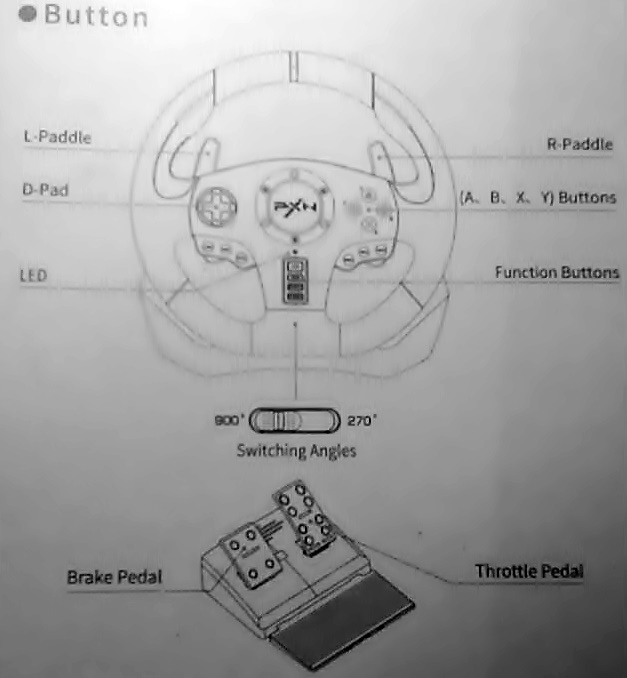
\includegraphics[scale=0.51]{img/steeringwheel.jpg}
	    %\caption{Diagram alur kerja}
	    \caption{Diagram Steering Wheel yang digunakan, \textit{Sumber : Buku Manual PXN Steering Wheel}}
	    \label{fig: 3_28}
    \end{figure}

	Konfigurasi kontroller yang perlu dilakukan adalah salah satunya melakukkan \textit{mapping} tombol - tombol dari keyboard ke tombol - tombol serta perangkat analog dari \textit{steering wheel controller} yang digunakan, seperti contohnya perangkat analog yang perlu dilakukan \textit{sampling} adalah pedal, \textit{sampling} yang dimaksud adalah melakukan pembagian data voltase analog yang ada di pedal menjadi nilai - nilai diskrit yang kemudian dapat dikonversikan ke kecepatan mobil, sesuai nilai - nilai diskrit yang didapatkan. Selain itu juga perlu dilakukan kalibrasi mode sudut dari steering wheel yang memiliki 2 macam mode, yaitu mode 270 derajat putaran, serta 900 derajat putaran. 
	Pada Tugas akhir ini, \textit{steering wheel} akan menggunakan mode 270 derajat, serta proses pergantian gigi \textit{(gear shift)} menggunakan proses manual tanpa kopling. Hal ini dikarenakan keterbatasan perangkat keras yang digunakan.
	
	\begin{figure}  [!htb]
	    \captionsetup{justification=centering}
	    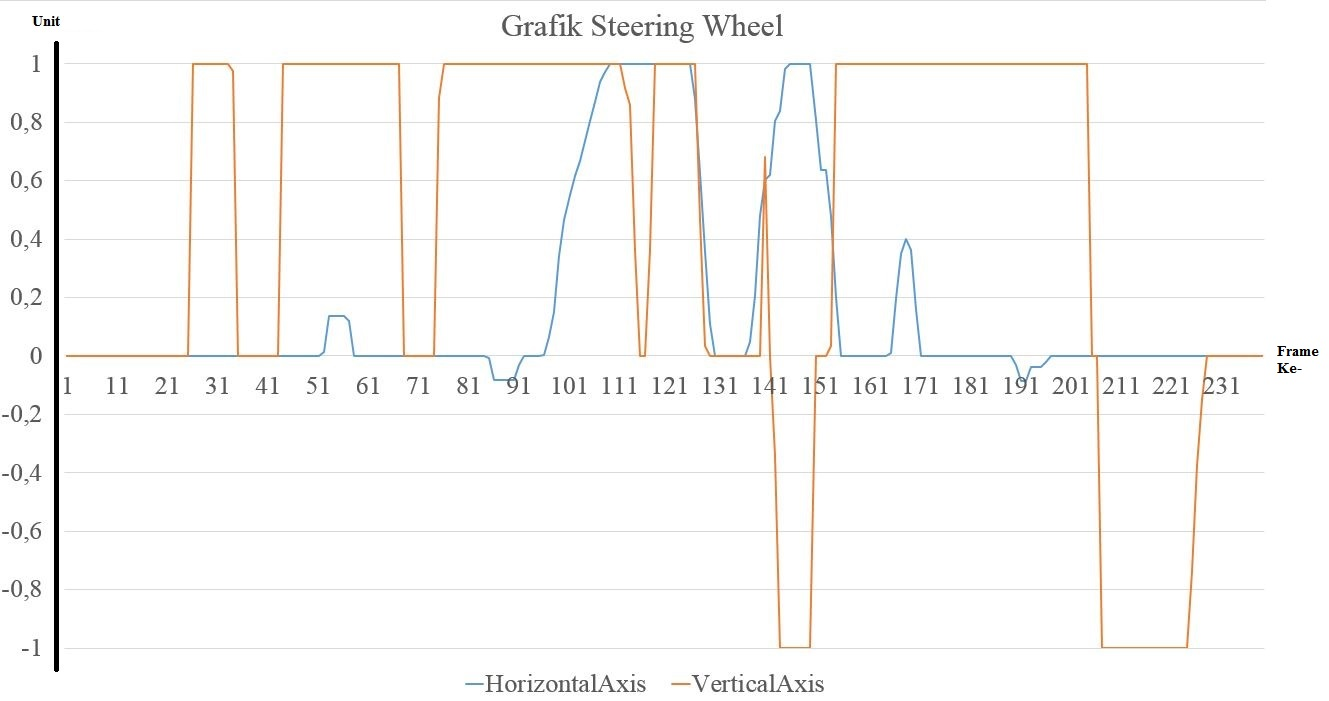
\includegraphics[scale=0.3]{img/driverinput.JPG}
	    %\caption{Diagram alur kerja}
	    \caption{Grafik hasil \textit{plotting} data \textit{input} pengemudi}
	    \label{fig: 3_29}
    \end{figure}
    
    Berikut pada gambar \ref{fig: 3_28} adalah \textit{key map} dari sistem simulator tugas akhir ini. proses kalibrasi pedal gas dan rem disambungkan ke \textit{vertical axis / axis y} dari \textit{unity controller}, maka bisa didapatkan nilai dari pedal atau rem tersebut, berupa data \textit{float} yang memiliki rentang 0 hingga 1. Sedangkan kalibrasi \textit{steering wheel} disambungkan dengan \textit{horizontal axis / axis x} dari \textit{unity controller}, yang memiliki data berupa \textit{float} dengan rentang -1 hingga 1.
    \par Kemudian, data \textit{float} tersebut, dapat dilakukan proses kalkulasi untuk mendapatkan sudut dari pedal gas dan rem, serta sudut dari \textit{steering wheel}, sehingga dapat dilakukan proses \textit{plotting} seperti berikut pada gambar \ref{fig: 3_29}
    
    Selain \textit{vertical axis} dan \textit{horizontal axis}, terdapat pula tombol - tombol lain dari \textit{steering wheel controller} yang digunakan. Yaitu tombol \textbf{X} untuk menyalakan mesin dari mobil \textit{(starter)}, selain itu ada tombol \textit{R-Paddle} dan \textit{L-Paddle} untuk menaikkan dan menurunkan gigi mesin secara berurutan. Proses ini, tidak memerlukan kopling, cukup menekan tombol \textit{L-R-Paddle} untuk menaikkan atau menurunkan gigi mobil.
    
    \par Di tengah \textit{steering wheel} juga terdapat \textit{switch} untuk mengganti mode \textit{steering} yaitu mode 270 derajat atau 900 derajat.
\section{Pembuatan Modul Pengambilan Data dengan \textit{Microcontroller}}
\label{microcontroller}
\vspace{1ex}

    \begin{figure}  [!htb]
	    \captionsetup{justification=centering}
	    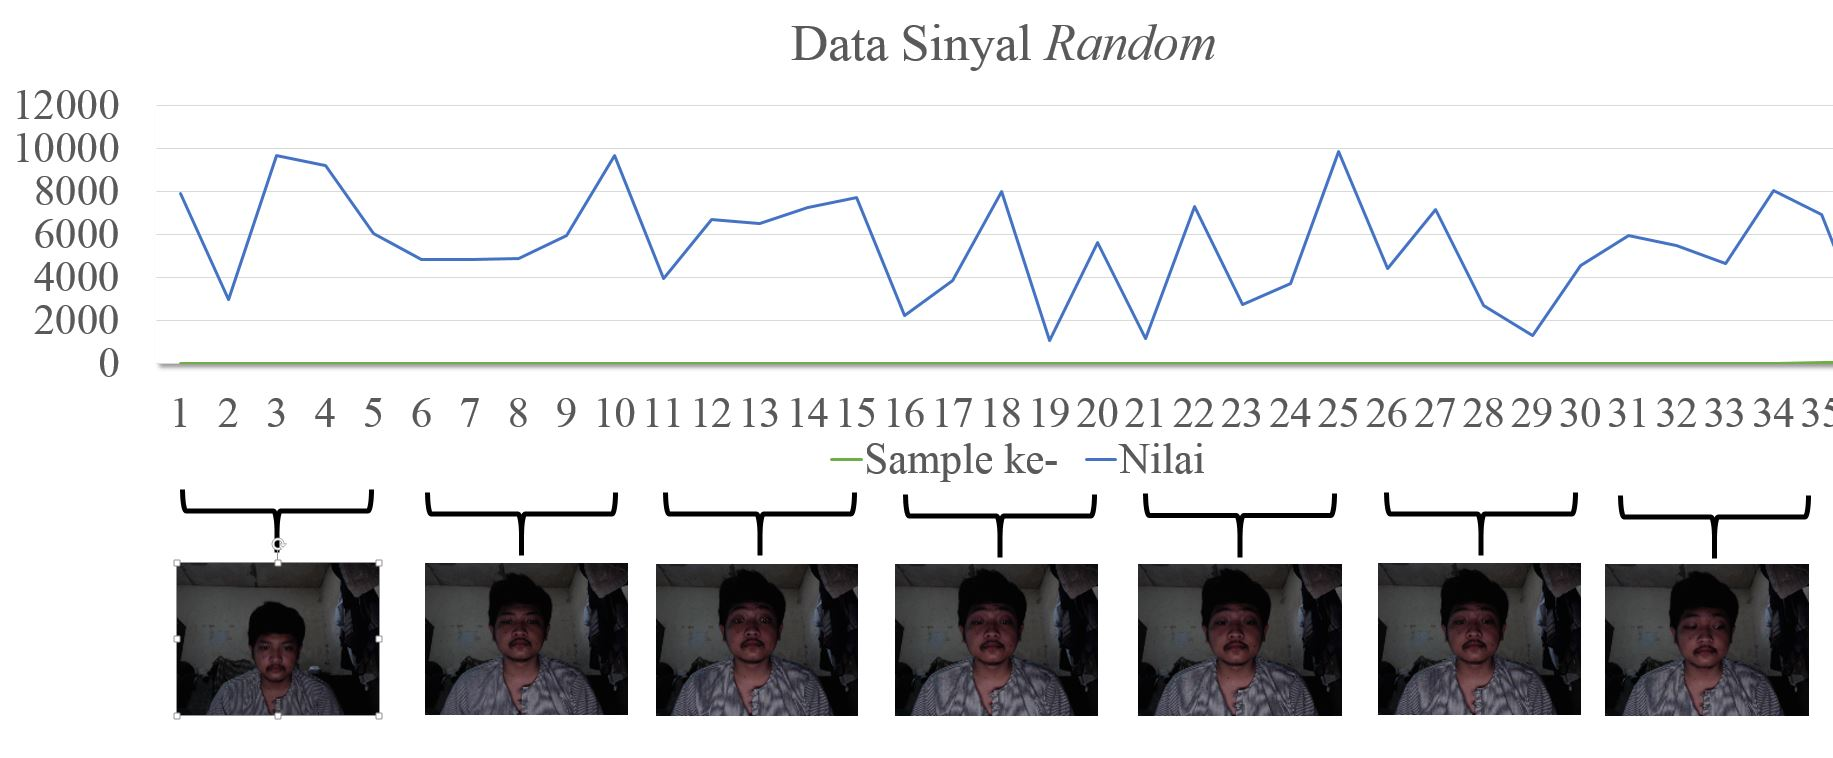
\includegraphics[scale=0.2]{img/sinyaldangambar.JPG}
	    %\caption{Diagram alur kerja}
	    \caption{Diagram Sinkronisasi \textit{capture rate} kamera dengan \textit{sampling rate} dari sensor arduino}
	    \label{fig: 3_30}
    \end{figure}
    
    Pembuatan modul pengambilan data serial seperti EEG dan ECG, dapat dilakukan menggunakan Arduino, sehingga perlu disiapkan port USB. Sedangkan pengambilan data berupa gambar wajah pengemudi menggunakan kamera, dapat disambungkan langsung ke \textit{Unity Game Engine} dan dapat langsung disimpan ke \textit{harddrive} komputer simulator. Hal ini dilakukan agar data yang masuk berupa gambar wajah pengemudi serta sinyal - sinyal yang di peroleh oleh \textit{microcontroller} dapat di lakukan pengolahan dan proses analisa.
    Perlu di perhatikan juga \textit{sampling rate} dari sistem pengambilan sinyal arduino, dengan \textit{capture rate} dari \textit{webcam}, kedua data tersebut perlu di sinkronkan dengan memperhatikan kedua nilai tersebut. \textit{Sampling rate} dari arduino disini bisa didapatkan dari \textit{datasheet} sensor yang digunakan, kemudian dilakukan kalkulasi dengan \textit{margin of error} yang disebabkan oleh kegagalan transmisi data dari arduino ke komputer simulator melalui kabel USB, agar didapatkan hasil yang dapat diterima. Sedangkan \textit{capture rate} dari kamera merupakan seberapa banyak gambar atau \textit{frame} yang diambil oleh kamera tiap \textit{frame} yang di proses oleh simulator. Pada Tugas Akhir ini, target capture rate adalah 1:1. Yang artinya, kamera akan mengambil gambar wajah pengemudi tiap frame game tersebut dijalankan. Berikut pada gambar \ref{fig: 3_30} adalah diagram dari penjelasan sinkronisasi kedua data tersebut, menjadi suatu modul analisis sinyal dengan gambar wajah.
    
\section{Penggabungan Seluruh Sistem Menjadi Satu Modul}
\vspace{1ex}
    Langkah terakhir adalah mengintegrasikan seluruh sistem menjadi satu modul yang utuh, supaya dapat melakukan pengolahan data dengan irisan waktu \textit{(t)} yang bersamaan. Keluaran yang diharapkan adalah, simulator dapat melakukan pengambilan data analog, data citra gambar, serta data - data internal simulasi secara bersamaan dan integrasi. Seperti yang dijelaskan pada bab \ref{logfilesystem} hingga bab \ref{steeringwheelconf}, Penggabungan Sub - sub modul, menjadi satu modul utuh adalah seperti berikut
    
    \begin{enumerate}[nolistsep]
	
	\item Sub-modul pengambilan data internal, mencakup :
	    \begin{enumerate}[nolistsep]
	        \item Sub-Modul Kecepatan Mobil
	            \begin{enumerate}
	                \item Kecepatan Vektor Sumbu \textit{x,y,z}
	                \item \textit{Magnitude} Kecepatan Vektor
	            \end{enumerate}
	        \item Sub-Modul Informasi Spasial
	            \begin{enumerate}
	                \item Posisi Relatif Mobil terhadap jalan
	                \item Sudut Euler dan \textit{6 Degree of Freedom} - Pitch, Yaw, Roll
	            \end{enumerate}
	        \item Sub-Modul Respon Pengemudi
	            \begin{enumerate}
	                \item Informasi Respon Pengemudi Ketika kendaraan keluar jalur
	                \item Informasi \textit{Input} dari Steering Wheel Controller (Sudut \textit{Steering Wheel} dan Nilai Tekanan Pedal Gas dan Rem)
	            \end{enumerate}
	    \end{enumerate}
	\item Sub-modul pengambilan data eksternal, mencakup :
	    \begin{enumerate}[nolistsep]
	        \item Sub-Modul Sinyal dan Citra Wajah
	            \begin{enumerate}
	                \item Sinyal dari sensor, bisa berupa ECG, EEG, atau EOG
	                \item Citra Wajah tiap frame dari kamera
	            \end{enumerate}
	    \end{enumerate}
	
	\end{enumerate}
    
Pada tugas akhir ini, sub - sub modul dibentuk berdasarkan kebutuhan proses pengujian, namun untuk riset kedepannya, proses pembuatan serta sinkronisasi data - data sub-modul bisa dapat dilakukan penyesuaian sesuai dengan kebutuhan riset tersebut yang menggunakan data dari simulator ini.
    
    
    
% GAMBAR KALIBRASI STEERING WHEEL
%\begin{figure} [!htb]
%	\captionsetup{justification=centering}
%	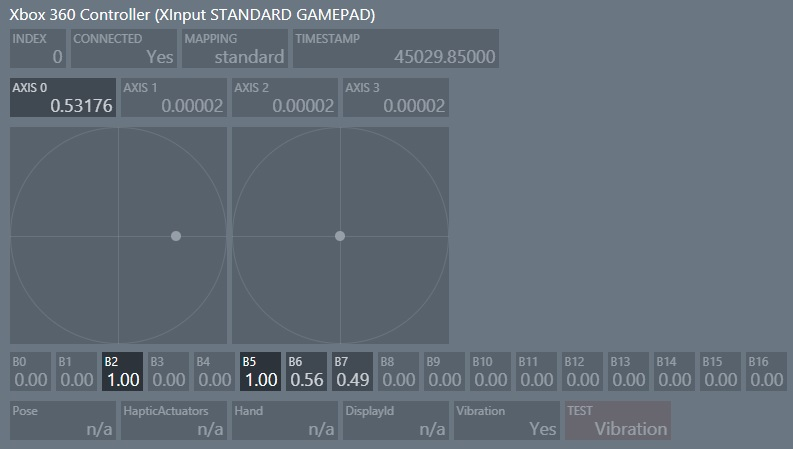
\includegraphics[scale=0.5]{img/steering-wheel-calibration.jpg}
%	\caption{Informasi Steering Wheel }
%	\label{fig: 3_7}
%\end{figure}

%GAMBAR FLOW CHART KOMUNIKASI PYTHON
\begin{figure}  [!htb]
	        \captionsetup{justification=centering}
	        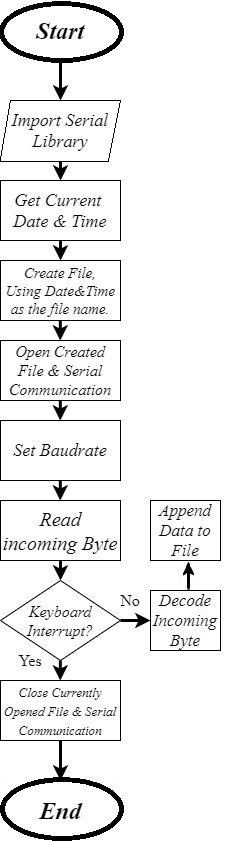
\includegraphics[scale=0.7]{img/serial-comm.jpg}
	        \caption{Diagram \textit{Flow Chart} Komunikasi Serial Melalui \textit{port} COM}
	        \label{fig: 3_25}
\end{figure}
\cleardoublepage
\chapter{PENGUJIAN DAN ANALISA}
\vspace{1ex}

\section*{}
Pada penelitian ini, dipaparkan hasil pengujian serta analisis dari desain sistem dan implementasi.  Data yang digunakan dalam pengujian data diambil dari IP Camera milik Dinas Perhubungan Kota Surabaya yang terpasang diseluruh lalu lintas Kota Surabaya. Pengambilan data video dilakukan di Surabaya Intelligent Transport System (SITS) dimana merupakan kantor Dinas Perhubungan khu- sus untuk pengendalian seluruh IP Camera lalu lintas yang tersebar di Kota Surabaya. Pengujian dilakukan dalam beberapa bagian se- bagai berikut:
\vspace{1ex}
\begin{enumerate}[nolistsep]
	\item Pengujian Peforma berdasarkan Lokasi
	\item Pengujian Peforma berdasarkan Kondisi.
	\item Pengujian Deteksi berdasarkan Objek Pelanggar.
	\item Pengujian Sistem
	
	\vspace{1ex}

\end{enumerate}
Dengan dilaksanakannya beberapa pengujian tersebut, sehingga dapat ditarik kesimpulan dari pelaksanaan tugas akhir ini.
\vspace{1ex}

\section{Pengujian Peforma berdasarkan Lokasi}
\vspace{1ex}

Pengujian peforma berdasarkan lokasi bertujuan untuk meng- etahui tingkat keakurasian pada YOLOv3 dan YOLOv3-tiny terha- dap lokasi yang memiliki karakteristik yang berbeda-beda. Pemilih- an lokasi didasarkan kondisi seperti sudut pandang kamera dan po- sisi kamera yang hampir dimiliki oleh semua kamera yang tersebar

\section{Pengujian Peforma berdasarkan Lokasi}
\vspace{1ex}

Pengujian peforma berdasarkan lokasi bertujuan untuk meng- etahui tingkat keakurasian pada YOLOv3 dan YOLOv3-tiny terha- dap lokasi yang memiliki karakteristik yang berbeda-beda. Pemilih- an lokasi didasarkan kondisi seperti sudut pandang kamera dan po- sisi kamera yang hampir dimiliki oleh semua kamera yang tersebar

\section{Pengujian Peforma berdasarkan Lokasi}
\vspace{1ex}

Pengujian peforma berdasarkan lokasi bertujuan untuk meng- etahui tingkat keakurasian pada YOLOv3 dan YOLOv3-tiny terha- dap lokasi yang memiliki karakteristik yang berbeda-beda. Pemilih- an lokasi didasarkan kondisi seperti sudut pandang kamera dan po- sisi kamera yang hampir dimiliki oleh semua kamera yang tersebar

\section{Pengujian Peforma berdasarkan Lokasi}
\vspace{1ex}

Pengujian peforma berdasarkan lokasi bertujuan untuk meng- etahui tingkat keakurasian pada YOLOv3 dan YOLOv3-tiny terha- dap lokasi yang memiliki karakteristik yang berbeda-beda. Pemilih- an lokasi didasarkan kondisi seperti sudut pandang kamera dan po- sisi kamera yang hampir dimiliki oleh semua kamera yang tersebar

\cleardoublepage
\chapter{PENUTUP}
\vspace{1ex}

\section{Kesimpulan}
\vspace{1ex}

Dari hasil pengujian yang sudah dilakukan dapat ditarik beberapa kesimpulan sebagai berikut:
\vspace{1ex}

\begin{enumerate}[nolistsep]

\item Tombol - tombol jumlah lajur pada \textit{Interface - Main Menu} telah berkorelasi dengan benar terhadap \textit{scene} yang dimuat
\item Pengujian pengambilan data kecepatan menghasilkan data berdasarkan kalkulasi vektor global, diperlukan pengujian untuk memverifikasi keakuratan data tersebut.
\item Pengujian pengambilan data spasial menghasilkan data relatif posisi mobil terhadap garis pinggir jalan, dapat disimpulkan data tersebut dapat digunakan untuk suplemen data pengujian pengambilan data \textit{response time}, diperlukan pengujian untuk memverifikasi keakuratan data tersebut 
\item Pengujian citra webcam memiliki \textit{performance cost} yang sangat tinggi, yaitu \textit{execution time} tiap framenya mencapai 250-550 milisekon, hal ini disebabkan oleh proses unity dalam melakukan \textit{encoding} data berupa \textit{texture} menjadi suatu citra. Permasalahan ini ada pada level perangkat keras (GPU dan CPU). Diperlukannya suatu kompromi antara \textit{performance} dan akurasi
\item Proses kalkulasi data serta berjalannya \textit{script} utama pada \textit{unity} tidak terlalu berpengaruh terhadap respon \textit{steering wheel}, nilai error mendekati 0 persen atau akurat hingga 5 angka dibelakang koma (0.000001\%)(gambar \ref{fig:4.8}) hal ini disebabkan oleh kecilnya \textit{performance cost} dari \textit{script} tersebut (20-100 milisekon).
\item Pengujian UX tidak konklusif, yang disebabkan oleh situasi dan kondisi pandemi \textit{COVID-19}. Diperlukannya pengujian UX dengan jumlah responden yang lebih banyak sehingga dapat mewakili target demografi pengguna yang dituju.

\end{enumerate}
\vspace{1ex}

\section{Saran}
\vspace{1ex}

Untuk pengembangan penelitian selanjutnya terdapat beberapa saran sebagai berikut :
\vspace{1ex}

\begin{enumerate}[nolistsep]
	
	\item Melakukan \textit{refactor} / penataan ulang terhadap struktur source code.
	\vspace{1ex}
	
	\item Mengurangi \textit{performance cost} dari source code.
	\vspace{1ex}
	
	\item Meningkatkan estetik dari simulator mulai dari UI, kualitas objek 3D, serta animasi - animasi atau detail - detail  lain yang dapat meningkatkan imersifitas dari simulator.
	
	\item Menambah kapabilitas dari simulator dengan menambah jenis data yang bisa diambil oleh simulator.
	\vspace{1ex}

    \item Melakukan survey terhadap pengguna untuk fitur yang perlu ditambahkan pada simulator ini
	\vspace{1ex}
	
	\item Melakukan survey kuesioner dengan jumlah responden yang lebih banyak agar mewakili target demografi pengguna yang dituju
	\vspace{1ex}

\end{enumerate}
\cleardoublepage

% Daftar pustaka
\renewcommand*\bibname{DAFTAR PUSTAKA}
\addcontentsline{toc}{chapter}{\bibname}
\titlespacing*{\chapter}{0pt}{-4ex}{2ex}
\appendix
\bibliographystyle{ieeetr}
\bibliography{TA}
\cleardoublepage

% Biografi penulis
\begin{center}
\Large\textbf{BIOGRAFI PENULIS}
\end{center}
\vspace{1ex}

\begin{wrapfigure}{L}{0.3\textwidth}
	\centering
	\vspace{-3ex}	
	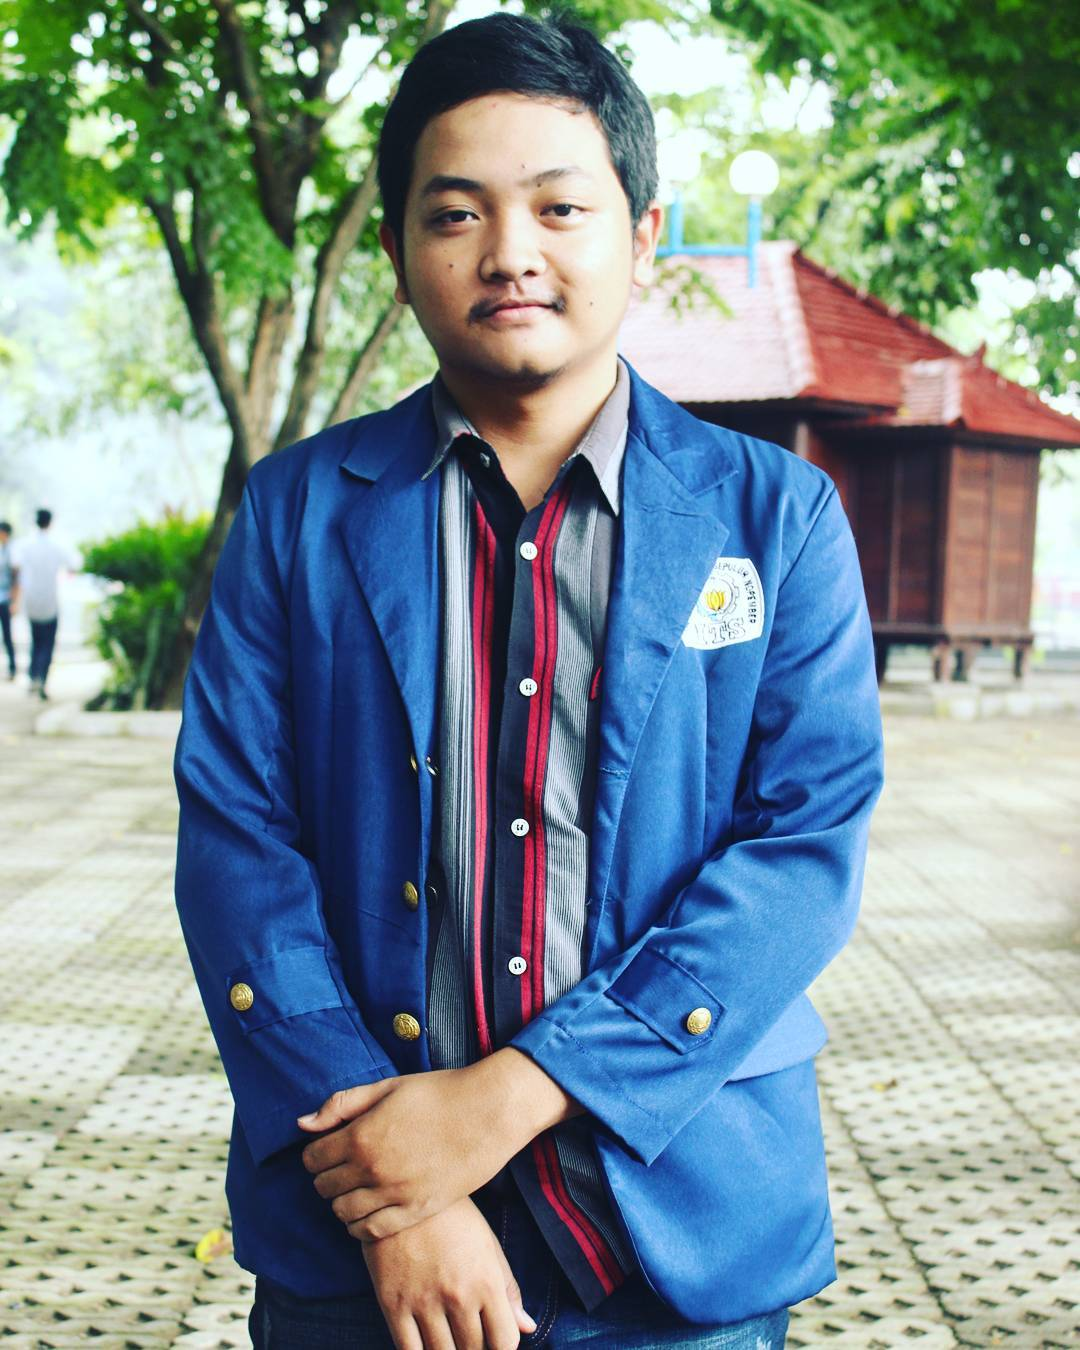
\includegraphics[width=0.31\textwidth]{img/Foto.jpg}
	\vspace{-4ex}
\end{wrapfigure}
\noindent
Penulis adalah salah satu mahasiswa S1 Departemen Teknik Komputer Fakultas Teknologi Elektro Institut Teknologi Sepuluh Nopember ITS. Penulis sangat tertarik dengan riset - riset yang berhubungan dengan sistem tertanam \textit{(embedded system)}, grafika komputer \textit{(computer graphics)}, dan visi komputer \textit{(Computer Vision)}.
\addcontentsline{toc}{chapter}{Biografi Penulis}
\cleardoublepage

\end{document}